\documentclass[12pt]{article}
\usepackage[utf8]{inputenc}
\usepackage[spanish]{babel}
\usepackage{csquotes}
\usepackage{geometry}
\usepackage{amsmath}
\geometry{a4paper, margin=1in}
\usepackage{setspace}
\usepackage{titling}
\usepackage{graphicx}
\usepackage{float}
\usepackage{longtable}
\usepackage{array}
\usepackage{comment} 
\usepackage{hyperref}
\usepackage{pgfgantt}
\usepackage{lmodern}
\usepackage{booktabs}
\usepackage{ragged2e}
\usepackage{tabularx}
\usepackage[
    backend=biber,
    style=ieee
]{biblatex}
\bibliography{src/referencias}
\usepackage{enumitem}
\usepackage{needspace}

\newenvironment{definicionmodulo}
{
    \begin{description}[
        style=multiline,
        leftmargin=3.5cm,
        labelwidth=3cm,
        labelsep=0.5cm,
        align=left,
        font=\bfseries,
        itemsep=0.9em,
        parsep=0pt,
        topsep=0.5em
    ]
}
{
    \end{description}
}

\newlist{elementosmodulo}{itemize}{1}
\setlist[elementosmodulo]{
    label=--,
    leftmargin=1.2em,
    itemsep=0.25em,
    parsep=0pt,
    topsep=0.35em
}




\addto\captionsspanish{%
    \renewcommand{\tablename}{Tabla}
}


\begin{document}

\begin{titlepage}
    \centering


    \LARGE\textbf{Universidad Técnica Federico Santa María}  \\[0.3cm]
    \begin{figure}[H]
        \centering
        
\includegraphics[width=0.4\linewidth]{images/Logo_UTFSM.png}
        
    \end{figure}
    \Large\textbf{Ingeniería Civil Telemática}     \\[2cm]


    \Huge\textbf{Sistema de transcripción de documentos antiguos mediante modelos de inteligencia artificial de código abierto en entornos computacionales limitados} \\[1.5cm]
    
    \large\textbf{Cristóbal Díaz Vilches} \\ [2.5cm]

    \large\textbf{Fecha:} 30-07-2026 \\
    \large\textbf{Versión:} 1.0 \\

    \vfill
\end{titlepage}


\newpage
\tableofcontents
\newpage
%==============================================================

%https://huggingface.co/PaddlePaddle/PaddleOCR-VL-1.6-GGUF/discussions/4
%error de paddle al crear caracteres fuera de UTF-8
%Mejor solución, utilizar otro modelo para la página

\section{Introducción}

En el marco de la implementación de la Ley N.º 21.180 sobre Transformación Digital del Estado, el Departamento de Tecnologías de la Información y las Comunicaciones de la Subsecretaría para las Fuerzas Armadas ha impulsado diversas iniciativas orientadas a modernizar la gestión documental institucional. Entre ellas se encuentra DocuDigital, proyecto destinado a preservar, centralizar y facilitar el acceso a la documentación histórica proveniente de las antiguas Subsecretarías de Guerra, Marina y Aviación.

Actualmente, DocuDigital se encuentra en su segunda versión y opera como una aplicación web para la consulta y recuperación de documentos digitalizados. La plataforma dispone de mecanismos de búsqueda basados en campos descriptivos, mediante los cuales es posible localizar distintos tipos de antecedentes administrativos.

\subsection{Problema a Resolver}

DocuDigital v2 presenta limitaciones asociadas a la heterogeneidad de los procesos de digitalización utilizados por las antiguas subsecretarías. Debido a que cada organismo definió de manera independiente sus propios criterios de registro y clasificación, documentos de naturaleza equivalente pueden contener campos distintos, estructuras inconsistentes o atributos sin correspondencia directa. Esta falta de estandarización dificulta la integración de la información en un repositorio centralizado y reduce la efectividad del actual mecanismo de búsqueda.

Adicionalmente, el sistema no dispone de información detallada sobre el contenido textual de los documentos digitalizados. En general, solo se conoce la categoría documental a la que pertenece cada archivo, sin contar con una descripción precisa de los antecedentes contenidos en su interior. En consecuencia, se dificulta la identificación de documentos específicos y aumenta el tiempo requerido para localizar antecedentes relevantes para la Subsecretaría para las Fuerzas Armadas.

\subsection{Acercamiento a la Solución }

Con el propósito de abordar las limitaciones de estandarización y recuperación de información presentes en DocuDigital v2, se está desarrollando de DocuDigital v3. Esta nueva versión conserva el acceso al repositorio histórico existente e incorporará funcionalidades para el ingreso de nuevos documentos y la ejecución de búsquedas avanzadas.

Dentro de esta evolución, el presente proyecto se centra en la incorporación de un sistema de transcripción y análisis documental basado en inteligencia artificial. La solución permitirá extraer el contenido textual de los documentos digitalizados y transformarlo en información estructurada, con el fin de homogeneizar, cuando la naturaleza del documento lo permita, los campos asociados a antecedentes de una misma categoría.

A partir de la información extraída, el sistema generará metadatos y descripciones de contenido que complementarán los datos actualmente disponibles. Esto permitirá mejorar los procesos de indexación y búsqueda, reducir la dependencia de campos definidos durante los antiguos procesos de digitalización y facilitar la identificación de los antecedentes contenidos en cada documento.

Debido a las restricciones de infraestructura tecnológica de la institución, la implementación deberá priorizar herramientas libres y de código abierto que sean compatibles con el hardware disponible. Asimismo, la solución deberá hacer un uso eficiente de los recursos computacionales y permitir el procesamiento de un volumen elevado de documentos, sin comprometer la estabilidad ni la continuidad operacional del sistema.

\subsection{Estado del Arte y de la Técnica}

\subsubsection{Reconocimiento Óptico de Caracteres a la comprensión documental}

El reconocimiento óptico de caracteres (OCR, \textit{Optical Character Recognition}) tiene como propósito convertir el texto presente en una imagen en una representación digital codifica y procesable por sistemas informáticos. Aunque esta definición puede sugerir una conversión directa entre píxeles y caracteres, el reconocimiento de documentos reales requiere distinguir regiones, identificar líneas o bloques, determinar el orden de lectura y reconstruir la relación entre los elementos de una página \cite{afkari2025transformers}, como se observa en la figura \ref{fig:ocr_dg}. Esta complejidad se debe a que los documentos no contienen únicamente texto continuo, sino que pueden integrar columnas, encabezados, tablas, fórmulas, figuras, sellos y anotaciones cuya posición contribuye a su significado \cite{subramani2021document}.

\begin{figure}[H]
    \centering
    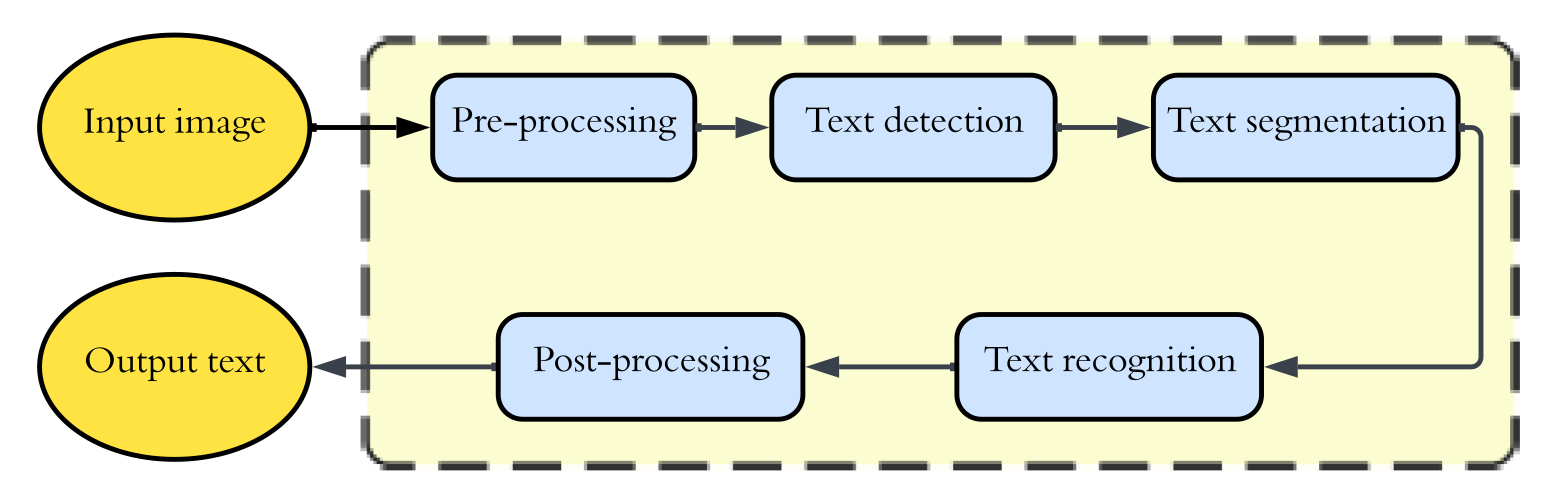
\includegraphics[width=0.5\linewidth]{images/estado del arte/ocr_diagram.png}
    \caption{Descripción general de un sistema OCR tradicional \cite{afkari2025transformers}}
    \label{fig:ocr_dg}
\end{figure}

La comprensión documental amplía el objetivo del OCR desde la transcripción hacia la recuperación conjunta del contenido y de su estructura lógica. Bajo este enfoque, una página puede transformarse en texto plano, Markdown, HTML o una representación estructurada que conserve títulos, párrafos, tablas y relaciones espaciales. Esta distinción es relevante porque una salida puede contener la mayoría de las palabras originales y, aun así, resultar poco útil si modifica el orden de lectura, mezcla columnas o destruye la organización de una tabla \cite{neudecker2021ocreval}. Por consiguiente, la calidad de un sistema documental no debe evaluarse exclusivamente por la presencia de caracteres correctos, sino también por su capacidad para preservar la forma en que la información está organizada.

El problema se vuelve más exigente en documentos escaneados, históricos o producidos bajo condiciones no controladas. El deterioro del papel, el bajo contraste, las manchas, la inclinación, las sombras y la resolución limitada alteran la apariencia de los caracteres y dificultan su separación respecto del fondo \cite{nguyen2021postocr}. Los errores generados en esta etapa se propagan hacia tareas posteriores, debido a que una fecha, un nombre o un identificador transcrito incorrectamente puede afectar la indexación, la búsqueda y la extracción automática de metadatos. En lenguas, tipografías o colecciones con pocos datos de entrenamiento, estas dificultades aumentan porque los modelos disponen de menor evidencia para representar las variaciones visuales y lingüísticas del dominio \cite{agarwal2024lowresource}.

\subsubsection{Preprocesamiento de documentos}

Antes de aplicar un modelo de reconocimiento, es posible reducir parte de la variabilidad visual mediante técnicas de preprocesamiento. Su finalidad no es modificar el contenido, sino facilitar la separación entre los trazos y el fondo para que el modelo reciba una entrada más uniforme. La ecualización adaptativa del histograma (AHE, Adaptive histogram equalization) mejora el contraste de manera local, lo que permite realzar regiones poco visibles sin aplicar la misma transformación a toda la página \cite{pizer1987ahe}. De forma complementaria, la binarización adaptativa calcula umbrales a partir del entorno de cada región y resulta apropiada cuando la iluminación o el color del fondo varían dentro del documento \cite{sauvola2000binarization}. Estas transformaciones no garantizan una mejora universal. Un aumento excesivo del contraste puede amplificar manchas, mientras que una binarización agresiva puede eliminar trazos finos, signos de puntuación o bordes de tablas. Por esta razón, la imagen original y cada perfil de preprocesamiento deben tratarse como configuraciones experimentales independientes, en lugar de asumir que una técnica es óptima para todas las páginas.

\subsubsection{Transformadores y Modelos Visión-Lenguaje}

Los sistemas OCR basados en aprendizaje profundo evolucionaron desde arquitecturas que combinaban redes convolucionales para extraer rasgos visuales y redes recurrentes para reconocer secuencias, hacia modelos fundamentados en transformadores. El mecanismo de autoatención de estas arquitecturas permite relacionar regiones distantes de una misma entrada y representar dependencias globales, lo que resulta útil cuando una línea, una columna o una celda debe interpretarse en función de otras zonas del documento \cite{afkari2025transformers}. Esta evolución también favoreció modelos generativos capaces de producir secuencias completas en lugar de clasificar caracteres de manera aislada.

Uno de estas arquitecturas es CRNN base-atention, la cual, combina la extracción de características visuales de una CNN, el modelado secuencial de una RNN y el cálculo de pesos contextuales de la atención para procesar datos complejos con alta precisión. En la figura \ref{fig:arch_trans} se observa un diagrama de su arquitectura. 

\begin{figure}[H]
    \centering
    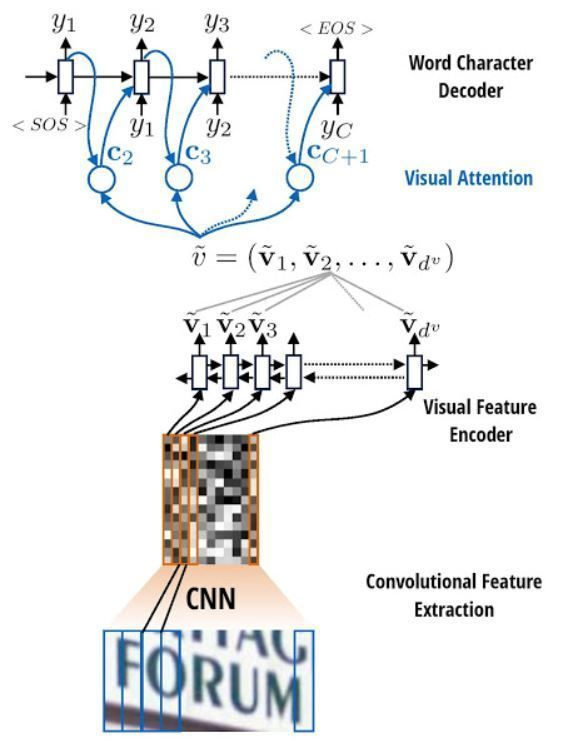
\includegraphics[width=0.4\linewidth]{images/estado del arte/arch_transformer.png}
    \caption{La arquitectura de un modelo CRNN base-attention \cite{afkari2025transformers}}
    \label{fig:arch_trans}
\end{figure}

Los modelos visión-lenguaje (VLM, \textit{Vision-Language Models}) integran representaciones visuales y lingüísticas dentro de una misma arquitectura. De manera general, un componente visual transforma la imagen en representaciones internas, un mecanismo de proyección las vincula con el espacio lingüístico y un modelo de lenguaje genera la respuesta condicionada por la imagen y por las instrucciones proporcionadas \cite{zhang2024vlmsurvey}, como se observa en la figura \ref{fig:vlm_ejem}. Aplicados a documentos, estos modelos pueden recibir una página completa y generar una secuencia que combine transcripción, orden de lectura y marcado estructural, reduciendo la necesidad de conectar manualmente múltiples módulos especializados.


\begin{figure}[H]
    \centering
    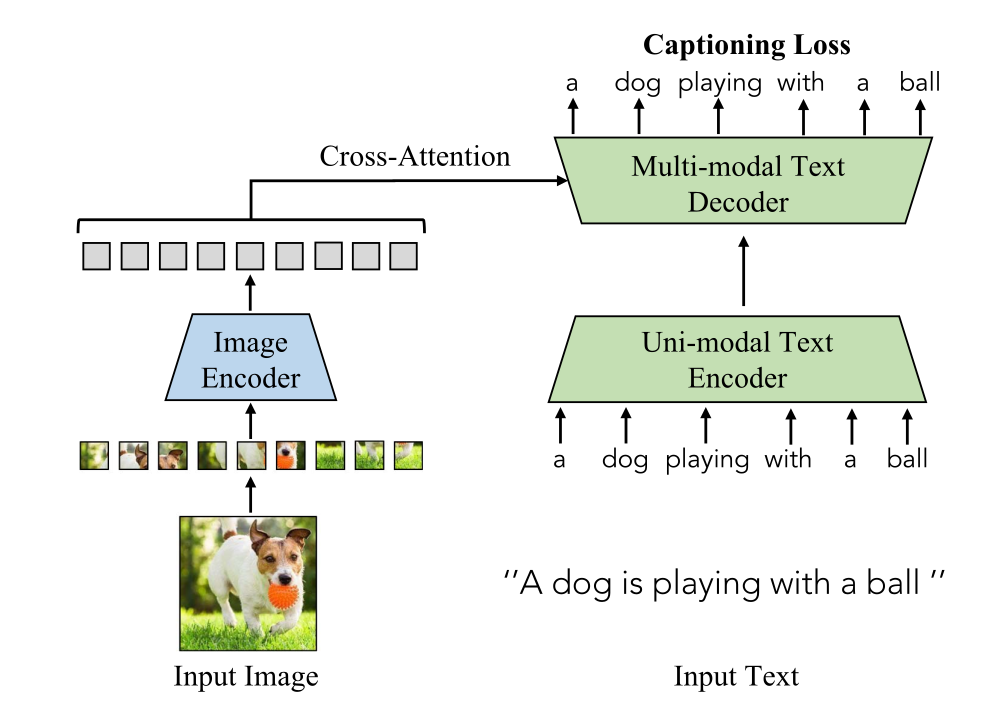
\includegraphics[width=0.5\linewidth]{images/estado del arte/vlm_ejem.png}
    \caption{Ilustración simplificada de la generación de COCA image-to-caption \cite{zhang2024vlmsurvey}}
    \label{fig:vlm_ejem}
\end{figure}

La principal ventaja de este enfoque es su flexibilidad, ya que un mismo modelo puede adaptarse mediante instrucciones a tareas de transcripción, descripción, extracción o conversión estructurada. Sin embargo, la generación lingüística también puede producir información plausible que no se encuentra respaldada por la imagen, fenómeno conocido como alucinación multimodal \cite{liu2024hallucination}. En consecuencia, una salida gramaticalmente correcta no constituye por sí sola evidencia de fidelidad documental. La validación debe realizarse mediante referencias verificadas y métricas que permitan detectar sustituciones, omisiones, contenido agregado y alteraciones estructurales.

\subsubsection{Modelos utilizados para el análisis documental}

Los modelos seleccionados representan distintas aproximaciones al análisis documental mediante inteligencia artificial. Para facilitar su comparación, se agrupan en dos familias: modelos visión-lenguaje de propósito general y modelos especializados en OCR y análisis documental. Esta clasificación permite relacionar la arquitectura de cada modelo con su nivel de especialización, tamaño y capacidad para procesar documentos multilingües.

\paragraph{Modelos visión-lenguaje de propósito general.}

Los modelos de la familia Qwen-VL fueron desarrollados para resolver tareas multimodales generales, entre las que se incluyen reconocimiento textual, comprensión de imágenes, análisis de documentos y razonamiento visual. \textbf{Qwen2-VL} introdujo un mecanismo de resolución dinámica que transforma imágenes de diferentes dimensiones en una cantidad variable de tokens visuales, evitando la necesidad de redimensionar todas las entradas a una resolución fija. Sobre esta base, Qwen2.5-VL-3B emplea aproximadamente 3 mil millones de parámetros y combina un codificador visual con un modelo de lenguaje autorregresivo, incorporando mecanismos de posicionamiento espacial que permiten conservar la relación entre texto, objetos y regiones de la imagen. La familia posee capacidades multilingües e incluye el procesamiento de texto en español, aunque su precisión documental depende de la calidad visual, la estructura de la página y la representación del idioma en los datos de entrenamiento \cite{wang2024qwen2vl}.

\begin{figure}[H]
    \centering
    \includegraphics[width=0.8\linewidth]{images/estado del arte/qwen3-vl.png}
    \caption{Arquitectura del modelo Qwen3-VL \cite{bai2025qwen3vl}.}
    \label{fig:qwen3-vl}
\end{figure}

\textbf{Qwen3-VL} amplía esta arquitectura mediante el mecanismo DeepStack, que incorpora al modelo de lenguaje características procedentes de diferentes niveles del codificador visual. Esta integración permite combinar detalles visuales locales con representaciones semánticas de mayor nivel. Asimismo, utiliza una variante mejorada de MRoPE para representar conjuntamente las dimensiones espaciales y secuenciales de la entrada. En este proyecto se considera la variante Qwen3-VL-2B, compuesta por aproximadamente 2 mil millones de parámetros. El modelo presenta capacidades multilingües para reconocimiento y comprensión visual, incluyendo el español; sin embargo, al tratarse de un VLM de propósito general, su rendimiento en transcripción y reconstrucción documental debe verificarse mediante una evaluación específica sobre los documentos de interés \cite{bai2025qwen3vl}.


La principal ventaja de esta familia reside en su versatilidad, dado que un mismo modelo puede reconocer texto, interpretar elementos visuales y responder instrucciones sobre el contenido. No obstante, esta generalidad implica un mayor espacio de tareas y no garantiza que la transcripción documental alcance el mismo nivel de precisión que un modelo entrenado específicamente para OCR.

\paragraph{Modelos especializados en OCR y análisis documental.}

A diferencia de los VLM de propósito general, los modelos especializados concentran su entrenamiento y arquitectura en la extracción de texto, la recuperación del orden de lectura y la representación de elementos estructurales, como tablas, fórmulas, gráficos y sellos.

\begin{figure}[H]
    \centering
    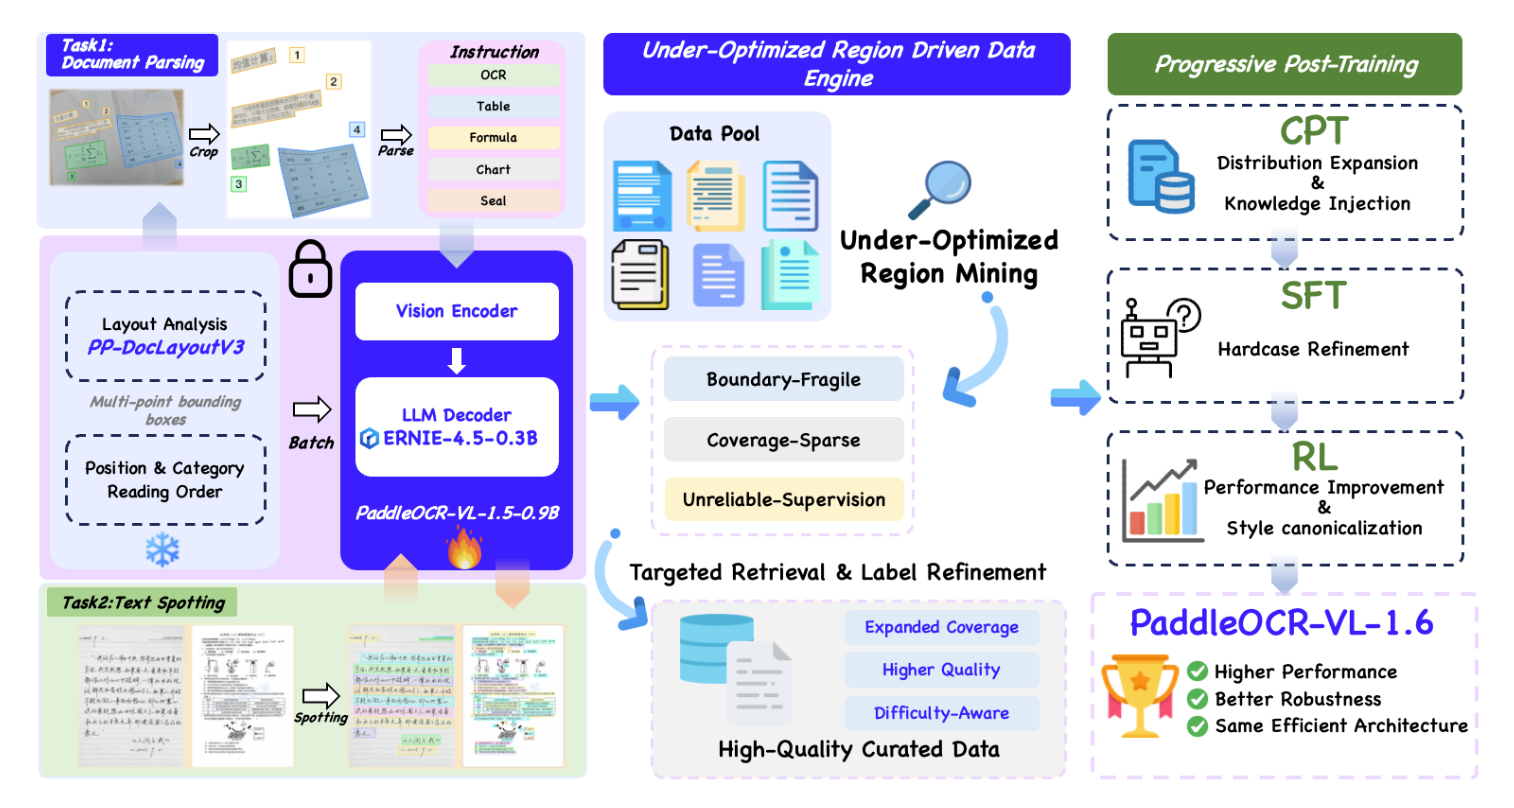
\includegraphics[width=0.7\linewidth]{images/estado del arte/paddle.png}
    \caption{Visión general del \textit{pipeline} PaddleOCR-VL-1.6 \cite{zhang2026paddleocrvl}.}
    \label{fig:paddle}
\end{figure}

\textbf{PaddleOCR-VL-1.6 }utiliza un \textit{pipeline} de dos etapas, como se observa en la figura \ref{fig:paddle}. En la primera, PP-Doc\allowbreak LayoutV3 analiza la distribución de la página y localiza sus regiones mediante cajas delimitadoras multipunto, lo que permite tratar documentos con perspectiva, curvatura o diseños irregulares. En la segunda etapa, cada región es procesada por PaddleOCR-VL\allowbreak-1.6-0.9B, un modelo de aproximadamente 0,9 mil millones de parámetros que integra un codificador visual de resolución nativa, un conector MLP adaptativo y el modelo lingüístico ERNIE-4.5-\allowbreak0.3B. El modelo reconoce texto, tablas, fórmulas, gráficos y sellos, mientras que un módulo de posprocesamiento reorganiza las predicciones en formatos como Markdown o JSON. La familia PaddleOCR-VL admite 109 idiomas e incluye explícitamente el español, por lo que posee soporte directo para documentos escritos en este idioma \cite{zhang2026paddleocrvl}.


\begin{figure}[H]
    \centering
    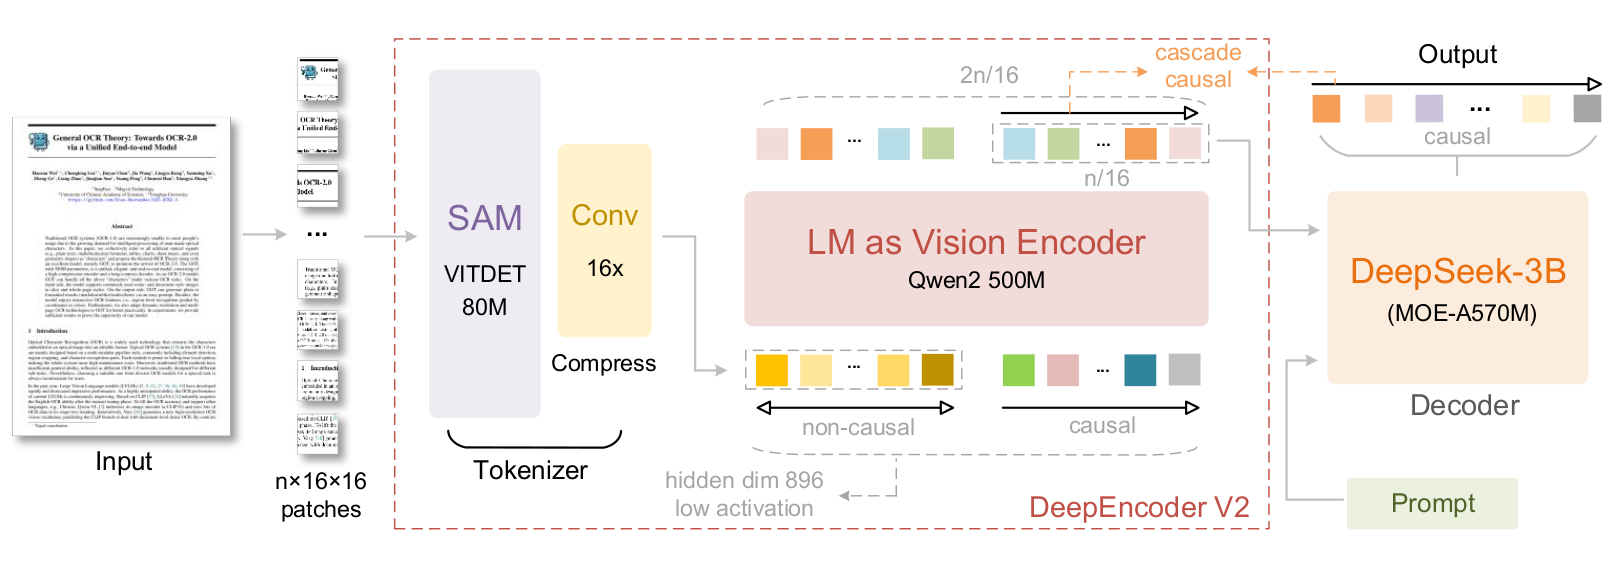
\includegraphics[width=0.7\linewidth]{images/estado del arte/deepseek-ocr2.png}
    \caption{Arquitectura del modelo DeepSeek-OCR 2 \cite{wei2026deepseekocr2}.}
    \label{fig:deepseek}
\end{figure}

\textbf{DeepSeek-OCR 2} emplea una arquitectura codificador--decodificador orientada a modelar el orden semántico de los documentos. Su componente DeepEncoder V2 combina un codificador visual compacto, atención bidireccional y consultas causales que reorganizan los tokens visuales antes de entregarlos al modelo de lenguaje. De esta manera, el procesamiento no queda restringido a un recorrido espacial fijo de izquierda a derecha y de arriba hacia abajo, sino que puede adaptarse a la estructura lógica de la página. Las representaciones obtenidas se entregan a un decodificador DeepSeek de 3 mil millones de parámetros con arquitectura \textit{Mixture-of-Experts}, encargado de generar autorregresivamente la transcripción o representación estructurada \cite{wei2026deepseekocr2}. El modelo se describe como multilingüe.

\begin{figure}[H]
    \centering
    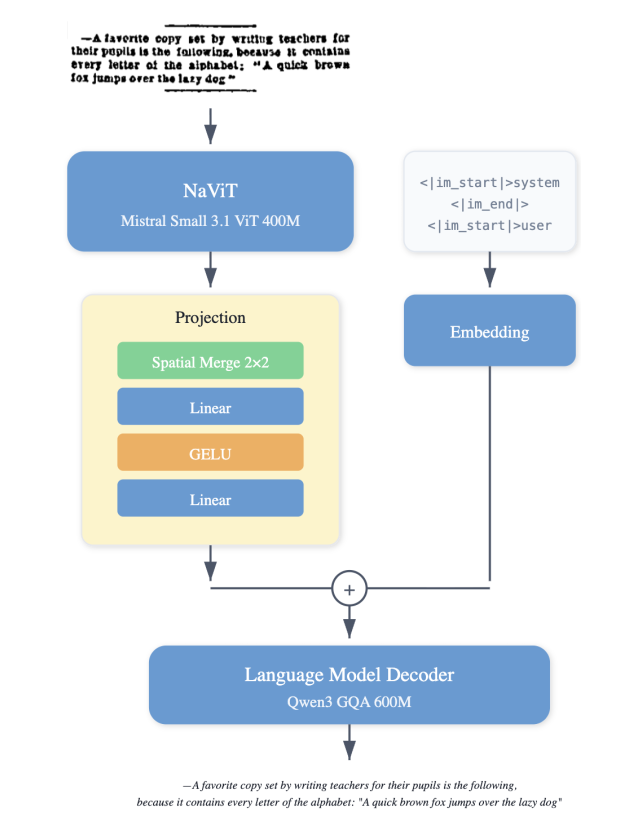
\includegraphics[width=0.5\linewidth]{images/estado del arte/lightOnOcr.png}
    \caption{Arquitectura del modelo LightOnOCR-2-1B \cite{taghadouini2026lightonocr}.}
    \label{fig:light}
\end{figure}

\textbf{LightOnOCR-2-1B }adopta un enfoque completamente \textit{end-to-end}, mediante el cual una página documental se transforma directamente en una secuencia textual estructurada sin ejecutar módulos independientes de detección, reconocimiento y reconstrucción del orden de lectura. El modelo posee aproximadamente 1.000 millones de parámetros y combina un codificador visual de resolución nativa inicializado desde Mistral-Small-3.1, un proyector multimodal que reduce en cuatro veces el número de tokens visuales mediante agrupación espacial, y un decodificador Qwen3 que genera la transcripción de forma autorregresiva. Su entrenamiento prioriza documentos escaneados, publicaciones científicas y lenguas europeas, con especial énfasis en francés. Por esta razón, el modelo dispone de capacidad para procesar texto en español por su base multilingüe y su cobertura de lenguas europeas \cite{taghadouini2026lightonocr}.

\begin{figure}[H]
    \centering
    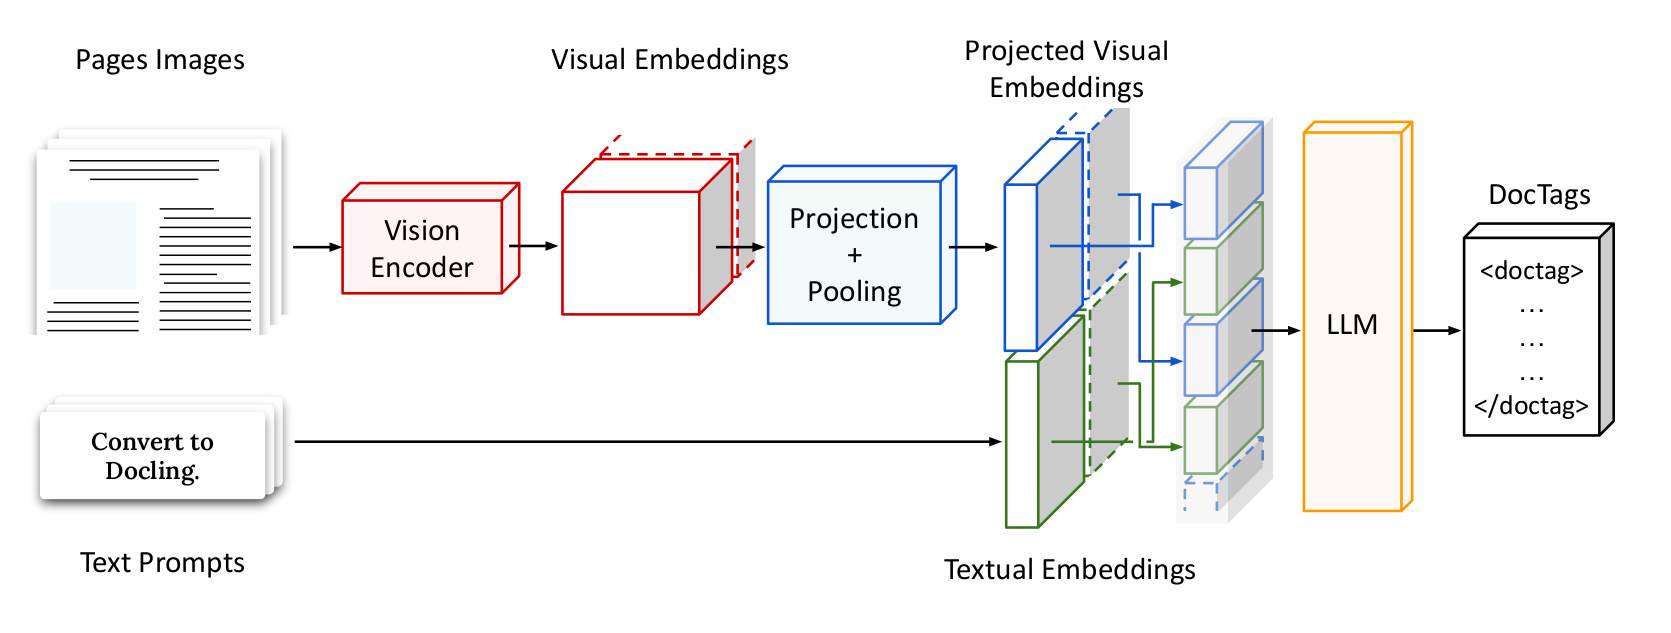
\includegraphics[width=0.5\linewidth]{images/estado del arte/docling.png}
    \caption{Arquitectura del modelo SmolDocling \cite{nassar2025smoldocling}.}
    \label{fig:docling}
\end{figure}

\textbf{Granite-Docling-258M} es un modelo visión-lenguaje \textit{end-to-end} de aproximadamente 258 millones de parámetros, especializado en convertir imágenes documentales en representaciones estructuradas mediante DocTags. Su arquitectura, que se observa en la figura \ref{fig:docling},se basa en IDEFICS3 e integra un codificador visual SigLIP2-base-patch16-512, encargado de extraer las características de la página, con un modelo de lenguaje Granite de 165 millones de parámetros que genera autorregresivamente el contenido, la estructura y la ubicación de elementos como texto, tablas, fórmulas, listas, código e imágenes. IBM lo describe como un modelo multilingüe \cite{ibm2025granitedoclingannouncement}.



En síntesis, los modelos analizados reflejan dos estrategias complementarias para el procesamiento documental. Los VLM de propósito general, representados por la familia Qwen-VL, ofrecen mayor flexibilidad para combinar reconocimiento textual, comprensión visual y razonamiento multimodal, mientras que los modelos especializados concentran su diseño en la extracción fiel del contenido, la recuperación del orden de lectura y la reconstrucción de elementos estructurales. Dentro de esta segunda familia, PaddleOCR-VL adopta un \textit{pipeline} por etapas, DeepSeek-OCR 2 reorganiza las representaciones visuales según la estructura semántica de la página, LightOnOCR realiza una conversión generativa completamente \textit{end-to-end} y Granite-Docling produce una representación compacta basada en DocTags. Por tanto, no existe una arquitectura universalmente superior, ya que la elección depende del equilibrio requerido entre precisión, conservación estructural, capacidad multilingüe, consumo de recursos y robustez frente a documentos complejos o degradados.


\subsubsection{Cuantización y ejecución en infraestructura local}

El uso local de modelos multimodales está condicionado por la memoria disponible y por la capacidad de cómputo del equipo. La cuantización reduce estos requerimientos al representar pesos o activaciones con menos bits que los utilizados durante el entrenamiento \cite{gholami2021quantization}. Esta reducción disminuye el tamaño del modelo y el tráfico de memoria, pero introduce una aproximación numérica que puede afectar la calidad de la salida. La degradación no es necesariamente gradual ni equivalente entre tareas, debido a que determinadas capas o distribuciones de valores son más sensibles a la reducción de precisión \cite{jin2024quantization}.

En OCR, la cuantización debe analizarse con especial cuidado porque diferencias pequeñas pueden modificar cifras, fechas, nombres propios o delimitadores estructurales. Por ello, el ahorro de memoria no puede considerarse suficiente para validar una configuración; debe relacionarse con métricas de fidelidad obtenidas sobre documentos representativos. Herramientas como \texttt{llama.cpp} permiten ejecutar modelos cuantizados en CPU, GPU o esquemas híbridos, facilitando su despliegue sobre hardware de propósito general \cite{sparrenberg2025llamacpp}. No obstante, el rendimiento efectivo depende del formato cuantizado, los kernels disponibles, la arquitectura del procesador, la aceleración por tarjeta de video y la distribución de la carga entre memoria y cómputo.


\subsubsection{Benchmarking y reproducibilidad experimental}

La comparación entre modelos requiere un benchmark que mantenga constantes los factores externos a la solución evaluada. Esto implica utilizar los mismos documentos, perfiles de preprocesamiento, parámetros de generación, condiciones de hardware y reglas de medición. Los marcos de evaluación de inferencia destacan que los resultados solo son comparables cuando la carga de trabajo y el procedimiento se encuentran definidos de manera explícita \cite{reddi2020mlperf}. Asimismo, cada ejecución debe conservar identificadores que permitan relacionar el documento, la página, el modelo, la cuantización, el perfil visual y la salida obtenida.

Bajo restricciones de hardware, el mejor modelo no es necesariamente aquel que obtiene la mayor precisión en una única métrica. Una configuración puede ser inviable si excede la memoria disponible, presenta tiempos de respuesta incompatibles con la operación o genera resultados inestables. Por tanto, la selección debe considerar simultáneamente fidelidad, latencia, consumo y robustez, manteniendo trazabilidad suficiente para reproducir cada comparación. Este criterio convierte el benchmark en un instrumento de decisión técnica y no únicamente en una clasificación de modelos.

\subsubsection{Evaluación de la fidelidad textual y estructural}

La evaluación combina métricas textuales, secuenciales y estructurales, debido a que los errores del análisis documental pueden manifestarse como caracteres sustituidos, palabras omitidas, contenido añadido, alteraciones del orden de lectura o reconstrucciones incorrectas de tablas. Antes de calcular los indicadores, la referencia y la predicción se someten al mismo proceso de normalización. Este procedimiento elimina etiquetas y tokens propios de cada modelo, transforma el contenido en texto plano, decodifica entidades, unifica mayúsculas y minúsculas, compacta espacios y aplica una tokenización común. De esta forma, las métricas textuales se concentran en la fidelidad del contenido y no en diferencias superficiales de formato.

La tasa de error de caracteres, o \textit{Character Error Rate} (CER), y la tasa de error de palabras, o \textit{Word Error Rate} (WER), cuantifican la distancia de edición entre la predicción y la referencia. Ambas consideran las sustituciones, eliminaciones e inserciones necesarias para transformar una secuencia en la otra, pero operan a diferente granularidad \cite{santos2019ocreval}:

\begin{equation}
    \mathrm{CER}
    =
    \frac{S_c+D_c+I_c}{N_c},
    \qquad
    \mathrm{WER}
    =
    \frac{S_w+D_w+I_w}{N_w},
    \label{eq:cer_wer}
\end{equation}

donde $S$, $D$ e $I$ corresponden a sustituciones, eliminaciones e inserciones, mientras que $N$ representa la longitud de la referencia. CER permite identificar alteraciones finas en fechas, cifras, identificadores y nombres propios, mientras que WER refleja el efecto de los errores sobre unidades léxicas completas. En ambos casos, un valor menor indica una transcripción más fiel. A partir de estas tasas se calculan además la exactitud de caracteres y la exactitud de palabras:

\begin{equation}
    \mathrm{Acc}_{c}=\max(0,1-\mathrm{CER}),
    \qquad
    \mathrm{Acc}_{w}=\max(0,1-\mathrm{WER}).
    \label{eq:character_word_accuracy}
\end{equation}

Estas exactitudes facilitan la interpretación y visualización de los resultados, ya que un valor mayor representa un mejor desempeño. Sin embargo, la aplicación de una cota inferior igual a cero oculta la magnitud de tasas de error superiores a uno; por esta razón, CER y WER se conservan como indicadores principales del error.

La precisión, la exhaustividad y la medida $F_1$ a nivel de tokens complementan las métricas de edición al distinguir entre contenido añadido y contenido omitido. Sea $C$ la intersección multiconjunto entre los tokens de la referencia y los de la predicción, de manera que se respeten las apariciones repetidas. Estas métricas se definen como \cite{powers2011evaluation}:

\begin{equation}
    P_{\mathrm{tok}}
    =
    \frac{|C|}{|\mathrm{Pred}|},
    \qquad
    R_{\mathrm{tok}}
    =
    \frac{|C|}{|\mathrm{GT}|},
    \qquad
    F_{1,\mathrm{tok}}
    =
    \frac{2P_{\mathrm{tok}}R_{\mathrm{tok}}}
         {P_{\mathrm{tok}}+R_{\mathrm{tok}}}.
    \label{eq:token_metrics}
\end{equation}

La precisión de tokens penaliza la sobregeneración, puesto que disminuye cuando la predicción contiene fragmentos que no están respaldados por la referencia. La exhaustividad penaliza las omisiones, mientras que $F_1$ proporciona un equilibrio entre ambas dimensiones. 

%Junto con estas métricas se registran los conteos \texttt{common\_tokens}, \texttt{extra\_tokens} y \texttt{missing\_tokens}, que representan, respectivamente, la cantidad de tokens coincidentes, añadidos y omitidos. Estos valores no constituyen métricas normalizadas independientes, sino indicadores diagnósticos que deben interpretarse junto con \texttt{gt\_token\_count} y \texttt{pred\_token\_count}.

La conservación del orden de lectura se evalúa mediante una adaptación de la subsecuencia común más larga, o \textit{Longest Common Subsequence} (LCS). Esta técnica permite determinar cuántos tokens de la referencia aparecen en la predicción manteniendo su orden relativo, aunque no se encuentren de forma contigua \cite{lin2004lcs}:

\begin{equation}
    \mathrm{RO}_{\mathrm{LCS}}
    =
    \frac{\operatorname{LCS}(\mathrm{GT},\mathrm{Pred})}{|\mathrm{GT}|}
    \label{eq:reading_order_lcs}
\end{equation}

Un valor igual a uno indica que todos los tokens de la referencia aparecen en el mismo orden relativo. 

%En este proyecto, LCS se emplea como un indicador diagnóstico del orden de lectura y no como una métrica OCR estandarizada. Además, debido a que no penaliza directamente todas las inserciones, debe analizarse en conjunto con la precisión de tokens y el conteo de tokens adicionales.

La evaluación de tablas requiere considerar tanto el contenido textual como las relaciones estructurales entre filas, columnas y celdas combinadas. 

%Para ello, se deben registrar \texttt{gt\_table\_count} y \texttt{pred\_table\_count}, correspondientes al número de tablas detectadas en la referencia y en la predicción. Estos conteos permiten identificar tablas omitidas o generadas incorrectamente antes de examinar su calidad individual.

La métrica \textit{Tree-Edit-Distance-based Similarity} (TEDS) compara las representaciones HTML de dos tablas como estructuras arbóreas. La medida considera las etiquetas de los nodos, las propiedades \texttt{rowspan} y \texttt{colspan}, y el contenido de las celdas \cite{zhong2020teds}:

\begin{equation}
    \mathrm{TEDS}
    =
    \max\left(
        0,
        1-
        \frac{
            \operatorname{TED}(T_{\mathrm{Pred}},T_{\mathrm{GT}})
        }{
            \max\left(
                |T_{\mathrm{Pred}}|,
                |T_{\mathrm{GT}}|
            \right)
        }
    \right).
    \label{eq:teds}
\end{equation}

TEDS entrega un valor entre cero y uno, donde un resultado mayor representa una mayor similitud conjunta de estructura y contenido. Su utilización permite penalizar errores que no son visibles mediante una comparación lineal del texto, como celdas desplazadas, combinaciones incorrectas o desalineaciones entre filas y columnas.

La evaluación tabular se complementa con las variantes \textit{GriTS Top} y \textit{GriTS Con}, pertenecientes al marco \textit{Grid Table Similarity} \cite{smock2023grits}. GriTS representa cada tabla como una matriz y alinea sus subestructuras mediante el problema de las subestructuras bidimensionales más similares. \textit{GriTS Top} evalúa la topología de la tabla, considerando la disposición de filas, columnas y expansiones de celdas, mientras que \textit{GriTS Con} mide la similitud del contenido textual de las celdas después de establecer su correspondencia estructural. Esta separación permite determinar si una predicción falla por reconstruir incorrectamente la grilla o por reconocer de manera deficiente el contenido de las celdas.

En conjunto, CER y WER evalúan la fidelidad de la transcripción; la precisión, la exhaustividad y $F_1$ distinguen entre contenido agregado y omitido; LCS examina la conservación del orden de lectura; y TEDS, GriTS Top y GriTS Con evalúan la reconstrucción tabular desde perspectivas complementarias. Por tanto, el desempeño de los modelos no se determina mediante un único indicador, sino mediante el análisis conjunto de sus errores textuales, secuenciales y estructurales.


\subsection{Referencias}
\printbibliography[heading=none]

\newpage

\section{Requisitos del Sistema}

%Los requisitos del sistema se derivan de las dificultades de estandarización, descripción y recuperación de la documentación histórica institucional. Su formulación corresponde a una etapa previa al diseño de la solución, por lo que establece las capacidades esperadas y las condiciones generales de operación sin definir componentes, tecnologías o mecanismos de implementación.

\subsection{Requisitos Funcionales}

\begin{enumerate}

    \item[\textbf{RF-01}] El sistema deberá permitir obtener el contenido textual
    presente en documentos digitalizados.

    \item[\textbf{RF-02}] El sistema deberá conservar, cuando la naturaleza del
    documento lo permita, el orden de lectura y la organización lógica de elementos
    como títulos, párrafos, columnas y tablas.

    \item[\textbf{RF-03}] El sistema deberá transformar la información recuperada
    en una representación procesable que permita identificar el contenido de cada
    documento.

    \item[\textbf{RF-04}] El sistema deberá generar información complementaria,
    como metadatos y descripciones de contenido, que apoye la homogeneización,
    indexación y búsqueda de los documentos.

    \item[\textbf{RF-05}] El sistema deberá admitir el análisis de documentos con
    diferentes estructuras, condiciones de digitalización y niveles de degradación
    visual.

    \item[\textbf{RF-06}] El proyecto deberá permitir comparar distintas
    alternativas de procesamiento documental mediante documentos representativos
    y criterios comunes de evaluación.

\end{enumerate}

\subsection{Requisitos No Funcionales}

\begin{enumerate}

    \item[\textbf{RNF-01}] La información generada deberá mantener fidelidad
    respecto del documento original, minimizando sustituciones, omisiones,
    incorporaciones de contenido y alteraciones estructurales.

    \item[\textbf{RNF-02}] La solución deberá utilizar eficientemente la capacidad
    de procesamiento y memoria disponible en la infraestructura institucional.

    \item[\textbf{RNF-03}] El sistema deberá permitir el procesamiento de un
    volumen elevado de documentos sin comprometer su estabilidad ni la continuidad
    operacional.

    \item[\textbf{RNF-04}] La implementación deberá priorizar herramientas libres
    y de código abierto que puedan ejecutarse dentro de la infraestructura
    institucional.

    \item[\textbf{RNF-05}] La selección de la alternativa de procesamiento deberá
    considerar conjuntamente la fidelidad de los resultados, el tiempo de
    procesamiento, el consumo de recursos y la estabilidad de ejecución.

    \item[\textbf{RNF-06}] Las comparaciones experimentales deberán ser
    reproducibles y mantener condiciones equivalentes para los documentos,
    configuraciones y recursos evaluados.

\end{enumerate}

\subsection{Requisitos Ambientales}

% Los requisitos ambientales describen las condiciones generales que deberá satisfacer el entorno de ejecución. Las capacidades mínimas definitivas deberán determinarse posteriormente mediante la evaluación experimental de las alternativas consideradas.

\subsubsection{Hardware}

\begin{enumerate}

    \item[\textbf{RA-H01}] La solución deberá poder ejecutarse utilizando la
    infraestructura computacional disponible en la institución, caracterizada por
    una capacidad limitada de procesamiento y memoria.

    \item[\textbf{RA-H02}] El sistema no deberá depender obligatoriamente de
    hardware especializado que no se encuentre disponible en el entorno
    institucional.

    \item[\textbf{RA-H03}] El entorno deberá disponer de capacidad suficiente para
    almacenar los documentos de entrada, los modelos de procesamiento y los
    resultados generados.

\end{enumerate}

\subsubsection{Software}

\begin{enumerate}

    \item[\textbf{RA-S01}] El entorno deberá admitir herramientas de procesamiento
    de imágenes, reconocimiento textual y análisis de estructura documental.

    \item[\textbf{RA-S02}] Las herramientas seleccionadas deberán ser compatibles
    con el sistema operativo y el hardware disponible en la institución.

    \item[\textbf{RA-S03}] El entorno deberá permitir la ejecución local de los
    modelos y mecanismos de procesamiento seleccionados.

    \item[\textbf{RA-S04}] El entorno de evaluación deberá permitir registrar y
    comparar la calidad de los resultados, los tiempos de ejecución y el consumo
    de recursos de cada alternativa.

    \item[\textbf{RA-S05}] Se deben ocupar herramientas de desarrollo utilizadas por el equipo de desarrollo de la institución.

\end{enumerate}

\section{Planificación del Proyecto}
\label{sec:planificacion}

%La planificación del proyecto se formula a partir del problema identificado y de los requisitos funcionales, no funcionales y ambientales definidos previamente. En esta etapa, el propósito de la planificación es establecer una ruta de trabajo que permita avanzar desde la caracterización de los documentos y del entorno institucional hasta la validación de una solución técnicamente viable.
%La planificación se organiza mediante un objetivo general, objetivos específicos, actividades e hitos. El objetivo general expresa el resultado global esperado, mientras que los objetivos específicos describen los resultados parciales necesarios para alcanzarlo. Cada objetivo específico se asocia con actividades y con un hito verificable que permite comprobar su cumplimiento.

\subsection{Objetivo General}
\label{subsec:objetivo_general}

Desarrollar y validar una solución de transcripción y análisis de documentos históricos digitalizados, basada en herramientas de código abierto y ejecutable en la infraestructura computacional disponible, capaz de recuperar con fidelidad el contenido textual y estructural y de generar información procesable que apoye la homogeneización, indexación y búsqueda documental en DocuDigital.

\subsection{Objetivos Específicos}
\label{subsec:objetivos_especificos}

\begin{enumerate}
    \item[\textbf{OE-01}] Caracterizar los documentos digitalizados considerados por el proyecto, identificando sus categorías, estructuras, condiciones de digitalización, niveles de degradación y elementos de información relevantes, mediante la conformación de un conjunto documental representativo.

    \item[\textbf{OE-02}] Definir un procedimiento reproducible para evaluar alternativas de procesamiento documental, estableciendo documentos de referencia, configuraciones experimentales, métricas de fidelidad y mecanismos para registrar tiempos de ejecución y consumo de recursos.

    \item[\textbf{OE-03}] Evaluar comparativamente alternativas de código abierto para la transcripción y el análisis documental bajo condiciones equivalentes, con el propósito de identificar configuraciones compatibles con las restricciones de infraestructura institucional.

    \item[\textbf{OE-04}] Implementar un prototipo funcional que permita procesar documentos digitalizados, recuperar su contenido textual y estructural y generar representaciones procesables, metadatos y descripciones de contenido.

    \item[\textbf{OE-05}] Validar el prototipo mediante documentos representativos y dentro del entorno computacional disponible, evaluando conjuntamente la fidelidad de los resultados, el tiempo de procesamiento, el consumo de recursos, la estabilidad y la reproducibilidad de la ejecución.
\end{enumerate}


\newcommand{\responsable}{\shortstack[c]{Cristóbal Díaz\\Vilches}}

\subsection{Hitos y Actividades}
\label{subsec:hitos_actividades}


\begingroup
\scriptsize
\renewcommand{\arraystretch}{1.15}
\setlength{\tabcolsep}{1.7pt}
\setlength{\LTleft}{0pt}
\setlength{\LTright}{0pt}
\setlength{\emergencystretch}{2em}
\sloppy

\begin{longtable}{
    >{\centering\arraybackslash}p{1.45cm}
    >{\RaggedRight\arraybackslash}p{6.0cm}
    >{\centering\arraybackslash}p{1.9cm}
    >{\centering\arraybackslash}p{1.65cm}
    >{\centering\arraybackslash}p{1.65cm}
    >{\centering\arraybackslash}p{0.95cm}
}
\caption{Actividades, tareas, resultados de producción e hitos del proyecto.}
\label{tab:hitos_actividades}\\

\toprule
\textbf{\shortstack{Act, \\ ...}} &
\textbf{Descripción resumida} &
\textbf{Responsable} &
\textbf{\shortstack{Fecha\\inicio}} &
\textbf{\shortstack{Fecha\\entrega}} &
\textbf{\shortstack{\% de\\logro}} \\
\midrule
\endfirsthead

\multicolumn{6}{c}{\tablename\ \thetable{} -- continuación} \\
\toprule
\textbf{\shortstack{Act, \\ ...}} &
\textbf{Descripción resumida} &
\textbf{Responsable} &
\textbf{\shortstack{Fecha\\inicio}} &
\textbf{\shortstack{Fecha\\entrega}} &
\textbf{\shortstack{\% de\\logro}} \\
\midrule
\endhead

\midrule
\multicolumn{6}{r}{Continúa en la página siguiente.} \\
\endfoot

\bottomrule
\endlastfoot

\addlinespace[3pt]
\multicolumn{6}{l}{\textbf{OE1 --- Caracterizar el dominio documental y sus restricciones}} \\
\midrule

\textbf{A1.1} &
\textbf{Contextualización institucional y formulación del problema.} &
\responsable &
01/06/2026 &
05/06/2026 &
\textbf{100\%} \\


\addlinespace[2pt]
\textbf{A1.2} &
\textbf{Caracterización del problema de transcripción y comprensión documental.} &
\responsable &
01/06/2026 &
05/06/2026 &
\textbf{100\%} \\


\addlinespace[2pt]
\textbf{A1.3} &
\textbf{Caracterización de restricciones ambientales y definición de requisitos.} &
\responsable &
01/06/2026 &
29/07/2026 &
\textbf{100\%} \\


\addlinespace[2pt]
\textbf{RP1} &
\textbf{Caracterización documental y requisitos del sistema.} &
\responsable &
01/06/2026 &
29/07/2026 &
\textbf{100\%} \\

\textbf{H1.1} &
\textbf{Problema, alcance y requisitos definidos.} &
\responsable &
29/07/2026 &
29/07/2026 &
\textbf{100\%} \\

\midrule
\addlinespace[3pt]
\multicolumn{6}{l}{\textbf{OE2 --- Definir una metodología reproducible de evaluación}} \\
\midrule

\textbf{A2.1} &
\textbf{Definición de referencias verificadas y normalización.} &
\responsable &
22/06/2026 &
03/07/2026 &
\textbf{100\%} \\

\addlinespace[2pt]
\textbf{A2.2} &
\textbf{Selección e implementación de métricas de evaluación.} &
\responsable &
23/06/2026 &
03/07/2026 &
\textbf{100\%} \\

\addlinespace[2pt]
\textbf{A2.3} &
\textbf{Diseño del experimento, captura de recursos y trazabilidad.} &
\responsable &
10/06/2026 &
03/07/2026 &
\textbf{100\%} \\


\addlinespace[2pt]
\textbf{A2.4} &
\textbf{Diseño e implementación del dashboard de resultados.} &
\responsable &
02/07/2026 &
29/07/2026 &
\textbf{100\%} \\

\addlinespace[2pt]
\textbf{RP2} &
\textbf{Protocolo de evaluación y diseño del benchmark.} &
\responsable &
10/06/2026 &
29/07/2026 &
\textbf{100\%} \\

\textbf{H2.1} &
\textbf{Metodología de evaluación disponible.} &
\responsable &
03/07/2026 &
03/07/2026 &
\textbf{100\%} \\

\textbf{H2.2} &
\textbf{Documentación de los diseños y métricas.} &
\responsable &
29/07/2026 &
29/07/2026 &
\textbf{100\%} \\

\midrule
\addlinespace[3pt]
\multicolumn{6}{l}{\textbf{OE3 --- Evaluar alternativas de procesamiento documental de código abierto}} \\
\midrule

\textbf{A3.1} &
\textbf{Investigación y preselección de modelos.} &
\responsable &
01/06/2026 &
19/06/2026 &
\textbf{100\%} \\

\addlinespace[2pt]
\textbf{A3.2} &
\textbf{Preparación de modelos, cuantizaciones y perfiles.} &
\responsable &
08/06/2026 &
26/06/2026 &
\textbf{100\%} \\

\addlinespace[2pt]
\textbf{A3.3} &
\textbf{Ejecución del benchmark comparativo.} &
\responsable &
10/06/2026 &
03/07/2026 &
\textbf{100\%} \\

\addlinespace[2pt]
\textbf{A3.4} &
\textbf{Análisis comparativo y selección.} &
\responsable &
17/06/2026 &
03/07/2026 &
\textbf{100\%} \\

\addlinespace[2pt]
\textbf{RP3} &
\textbf{Evaluación comparativa de modelos y configuraciones.} &
\responsable &
01/06/2026 &
03/07/2026 &
\textbf{100\%} \\

\textbf{H3.1} &
\textbf{Herramienta de visualización y comparación de resultados.} &
\responsable &
03/07/2026 &
03/07/2026 &
\textbf{100\%} \\

\textbf{H3.2} &
\textbf{Alternativa de procesamiento seleccionada.} &
\responsable &
03/07/2026 &
03/07/2026 &
\textbf{100\%} \\

\textbf{H3.3} &
\textbf{Benchmark integrado y reproducible.} &
\responsable &
26/06/2026 &
26/06/2026 &
\textbf{100\%} \\

\midrule
\addlinespace[3pt]
\multicolumn{6}{l}{\textbf{OE4 --- Implementar un prototipo de transcripción y análisis documental}} \\
\midrule

\textbf{A4.1} &
\textbf{Diseño de arquitectura, módulos e interfaces.} &
\responsable &
06/07/2026 &
29/07/2026 &
\textbf{100\%} \\


\addlinespace[2pt]
\textbf{A4.2} &
\textbf{Implementación del flujo de preprocesamiento e inferencia.} &
\responsable &
08/07/2026 &
20/07/2026 &
\textbf{100\%} \\

\addlinespace[2pt]
\textbf{A4.3} &
\textbf{Generación de salida estructurada, metadatos y descripciones.} &
\responsable &
20/07/2026 &
02/10/2026 &
\textbf{50\%} \\

\addlinespace[2pt]
\textbf{A4.4} &
\textbf{Integración local y manejo robusto de ejecuciones.} &
\responsable &
13/07/2026 &
21/08/2026 &
\textbf{80\%} \\

\addlinespace[2pt]
\textbf{RP4} &
\textbf{Prototipo funcional de procesamiento documental.} &
\responsable &
08/07/2026 &
23/10/2026 &
\textbf{82.5\%} \\

\textbf{H4.1} &
\textbf{Procesamiento documental de extremo a extremo.} &
\responsable &
20/07/2026 &
20/07/2026 &
\textbf{100\%} \\

\textbf{H4.2} &
\textbf{Servicio OCR, CLI y API operativos.} &
\responsable &
23/07/2026 &
23/07/2026 &
\textbf{100\%} \\

\midrule
\addlinespace[3pt]
\multicolumn{6}{l}{\textbf{OE5 --- Validar y documentar la solución en el entorno institucional}} \\
\midrule

\textbf{A5.1} &
\textbf{Preparación del conjunto final de validación.} &
\responsable &
22/06/2026 &
06/11/2026 &
\textbf{50\%} \\

\addlinespace[2pt]
\textbf{A5.2} &
\textbf{Validación de fidelidad y eficiencia.} &
\responsable &
15/06/2026 &
20/11/2026 &
\textbf{66.7\%} \\

\addlinespace[2pt]
\textbf{A5.3} &
\textbf{Pruebas de estabilidad y procesamiento por lotes.} &
\responsable &
20/07/2026 &
27/11/2026 &
\textbf{60\%} \\

\addlinespace[2pt]
\textbf{A5.4} &
\textbf{Documentación técnica, académica y recomendaciones.} &
\responsable &
21/07/2026 &
11/12/2026 &
\textbf{75\%} \\

\addlinespace[2pt]
\textbf{RP5} &
\textbf{Solución validada y documentación técnica.} &
\responsable &
15/06/2026 &
11/12/2026 &
\textbf{62.9\%} \\

\textbf{H5.1} &
\textbf{Solución validada y documentada.} &
\responsable &
11/12/2026 &
11/12/2026 &
\textbf{0\%} \\

\end{longtable}

\endgroup



\subsection{Carta Gantt}

\begin{figure}[H]
    \centering
    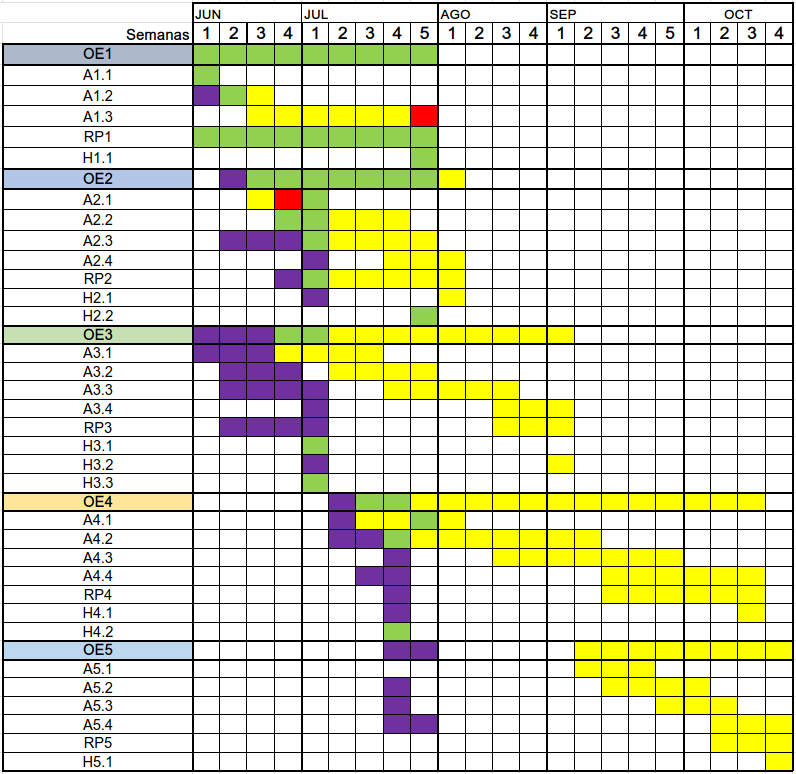
\includegraphics[width=1.0\linewidth]{images/Gantt.png}
    \caption{Carta Gantt}
    \label{fig:gantt}
\end{figure}

\begin{figure}[H]
    \centering
    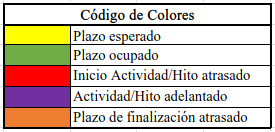
\includegraphics[width=0.4\linewidth]{images/coloresGantt.png}
    \caption{Codigo de colores de Carta Gantt}
    \label{fig:colorGantt}
\end{figure}


\section{Arquitectura del Sistema}

\subsection{Diagrama de Contexto}

\begin{figure}[H]
    \centering
    \includegraphics[width=0.7\linewidth]{images/Contexto.png}
    \caption{Diagrama de contexto del sistema propuesto.}
    \label{fig:diagrama_contexto_sistema}
\end{figure}

Como se observa en la figura \ref{fig:diagrama_contexto_sistema}, el diagrama de contexto el Sistema Coordinador concentra la interacción con los usuarios, el control de acceso y la administración documental, mientras que el Servidor OCR ejecuta el procesamiento especializado. Ambos sistemas se comunican mediante una API y utilizan la base de datos institucional para consultar y almacenar la información necesaria.

Los usuarios interactúan con el front end del Sistema Coordinador. Las solicitudes autorizadas son enviadas al Servidor OCR, cuyos resultados son registrados y posteriormente puestos a disposición del usuario.

Este enfoque permite separar la lógica de gestión del procesamiento OCR, facilitando la sustitución de modelos, la administración de tareas y la adaptación del sistema a los recursos disponibles, \textbf{permitiendo la posibilidad de tener Servidores OCR en paralelo}.


\subsection{Diagrama de Arquitectura}

La arquitectura del sistema se compone de un \textbf{Sistema Coordinador}, uno o más \textbf{OCR Server}, un servidor institucional \textbf{MySQL} y una base de datos local \textbf{SQLite}, como se observa en la figura \ref{fig:arquitectura}. El Sistema Coordinador centraliza la interacción con los usuarios, la preparación de los documentos, la gestión distribuida de las tareas y la persistencia de los resultados. Los OCR Server actúan como nodos independientes de procesamiento, permitiendo ejecutar tareas en paralelo entre distintas instancias.

\begin{figure}[H]
    \centering
    \includegraphics[width=0.7\linewidth]{images/Arquitectura.png}
    \caption{Diagrama de arquitectura del sistema propuesto.}
    \label{fig:arquitectura}
\end{figure}



Dentro del Sistema Coordinador, el módulo \textbf{M1: Portal Web y Control de Acceso} permite autenticar a los usuarios, solicitar nuevos procesamientos y consultar las tareas registradas. El módulo \textbf{M2: Catálogo Estructural MySQL} obtiene los metadatos del servidor institucional y mantiene en SQLite una representación actualizada de sus bases de datos, tablas y columnas. Esta información es utilizada por el portal y por los demás módulos para validar las operaciones realizadas sobre MySQL.

El módulo \textbf{M3: Preparación de Lotes Documentales} recibe la solicitud de procesamiento, valida la tabla, la columna documental y el rango seleccionado, y genera una nueva tarea. La tarea es entregada al módulo \textbf{M4: Gestión y Orquestación Distribuida de Tareas}, encargado de dividir el lote en elementos individuales, registrar su estado en SQLite y distribuir los documentos entre los OCR Server disponibles.

Cada OCR Server dispone del módulo \textbf{M5: API de Integración con OCR Server}, que recibe las solicitudes del Sistema Coordinador y traduce las respuestas del servicio. El módulo \textbf{M6: Administración del Servicio OCR} controla el estado operativo, el modelo activo y la ejecución interna del servidor. Finalmente, el módulo \textbf{M7: Procesamiento e Inferencia Documental} ejecuta la transcripción del documento y devuelve el contenido reconocido, los metadatos, los tiempos de ejecución y los errores detectados.

Los resultados obtenidos son enviados nuevamente al Sistema Coordinador. El módulo \textbf{M4} actualiza el progreso de la tarea y entrega los resultados al módulo \textbf{M8: Persistencia y Trazabilidad de Resultados}. Este último consulta la estructura de destino, relaciona cada resultado con su documento de origen y registra la transcripción final en MySQL sin eliminar la información original.

SQLite mantiene el catálogo estructural, el registro de los OCR Server y el estado de las tareas, mientras que MySQL conserva los documentos originales y los resultados procesados. La utilización de múltiples OCR Server permite aumentar la capacidad de procesamiento, distribuir la carga y continuar las tareas disponibles cuando una instancia se encuentra ocupada o fuera de servicio.


\subsection{Enumeración de Módulos}
\label{subsec:enumeracion_modulos}

\begin{table}[H]
    \centering
    \footnotesize
    \renewcommand{\arraystretch}{1.15}
    \caption{Módulos de la arquitectura del sistema.}
    \label{tab:enumeracion_modulos}

    \begin{tabularx}{\textwidth}{
        >{\raggedright\arraybackslash}p{0.30\textwidth}
        >{\raggedright\arraybackslash}X
        >{\centering\arraybackslash}p{0.13\textwidth}
    }
        \toprule
        \textbf{Módulo} & \textbf{Propósito} & \textbf{Sección} \\
        \midrule

        M1: Portal web y acceso &
        Proporcionar acceso autenticado y las vistas de operación. &
        \ref{subsec:modulo_m1} \\

        M2: Catálogo estructural MySQL &
        Registrar en SQLite la estructura de los servidores MySQL. &
        \ref{subsec:modulo_m2} \\

        M3: Preparación de lotes &
        Seleccionar y validar los registros que serán procesados. &
        \ref{subsec:modulo_m3} \\

        M4: Gestión de tareas &
        Controlar la creación, ejecución, seguimiento y reprocesamiento. &
        \ref{subsec:modulo_m4} \\

        M5: API de integración OCR &
        Comunicar el Sistema Coordinador con OCR Server. &
        \ref{subsec:modulo_m5} \\

        M6: Administración del servicio OCR &
        Controlar el daemon, los modelos, los estados y los registros técnicos. &
        \ref{subsec:modulo_m6} \\

        M7: Procesamiento e inferencia &
        Procesar imágenes y PDF mediante el modelo activo. &
        \ref{subsec:modulo_m7} \\

        M8: Persistencia y trazabilidad &
        Registrar los resultados y asociarlos con los documentos de origen. &
        \ref{subsec:modulo_m8} \\

        \bottomrule
    \end{tabularx}
\end{table}

\subsection{Matriz de Requisitos Funcionales y Módulos}
\label{subsec:matriz_requisitos_modulos}


\begin{table}[H]
    \centering
    \footnotesize
    \renewcommand{\arraystretch}{1.15}
    \caption{Matriz de requisitos funcionales y módulos.}
    \label{tab:matriz_requisitos_modulos}

    \begin{tabular}{c|cccccccc}
        \toprule
        \textbf{Requisito}
        & \textbf{M1} & \textbf{M2} & \textbf{M3} & \textbf{M4}
        & \textbf{M5} & \textbf{M6} & \textbf{M7} & \textbf{M8} \\
        \midrule
        RF1 & X &   &   &   &   &   &   &   \\
        RF2 & X &   &   &   & X & X &   &   \\
        RF3 &   & X &   &   &   &   &   &   \\
        RF4 & X & X & X &   &   &   &   &   \\
        RF5 & X &   & X & X & X &   &   & X \\
        RF6 &   &   &   &   & X & X &   &   \\
        RF7 &   &   &   &   & X & X & X &   \\
        RF8 &   & X &   & X &   &   &   & X \\
        \bottomrule
    \end{tabular}
\end{table}


\section{Módulos}
\label{sec:modulos}

Los módulos M1 a M4 y M8 forman parte del Sistema Coordinador, mientras que los módulos M5 a M7 corresponden a las funciones proporcionadas por OCR Server. Su interacción permite seleccionar documentos almacenados en MySQL, administrar su procesamiento, ejecutar la transcripción y conservar los resultados obtenidos.


% ============================================================
% MÓDULO M1
% ============================================================

\Needspace{8\baselineskip}
\subsection{Definición del Módulo: Portal Web y Control de Acceso (M1)}
\label{subsec:modulo_m1}

\begin{definicionmodulo}

\item[Propósito] El módulo Portal Web y Control de Acceso constituye el punto de interacción entre los usuarios y el Sistema Coordinador. Su propósito es proporcionar una interfaz protegida para consultar los servicios disponibles, seleccionar información almacenada en MySQL, iniciar tareas de procesamiento documental y revisar su estado. También debe asegurar que únicamente los usuarios autorizados puedan acceder a las funciones internas de la aplicación.

\item[Alcance] El módulo comprende la vista de ingreso, la vista principal, la selección de bases de datos y tablas, la configuración del procesamiento, la lista de tareas y el detalle de cada tarea. Incluye la creación y conservación de la sesión, la protección de las rutas internas, la presentación del estado de MySQL y OCR Server y la navegación entre las distintas vistas del portal. No ejecuta directamente consultas estructurales complejas, tareas OCR ni escrituras sobre los datos institucionales.

\item[Dependencias]
\begin{elementosmodulo}
    \item Servicio MySQL, utilizado para autenticar al usuario y validar que posea permisos administrativos.
    \item Módulo Catálogo Estructural MySQL, utilizado para presentar las bases de datos, tablas y columnas disponibles.
    \item Módulo Preparación de Lotes Documentales, encargado de validar la selección realizada por el usuario.
    \item Módulo Gestión y Orquestación de Tareas, utilizado para crear y consultar las tareas.
    \item Módulo API de Integración con OCR Server, utilizado para consultar la disponibilidad del servicio OCR.
\end{elementosmodulo}

\item[Supuestos]
\begin{elementosmodulo}
    \item El usuario dispone de credenciales válidas para el servidor MySQL seleccionado.
    \item Las credenciales utilizadas poseen permisos administrativos suficientes para operar sobre las bases de datos autorizadas.
    \item El estado de MySQL y OCR Server puede ser consultado desde el back end.
\end{elementosmodulo}

\item[Restricciones]
\begin{elementosmodulo}
    \item La vista de ingreso será la única vista accesible sin una sesión válida.
    \item Todo intento de acceder directamente a una ruta interna deberá redirigir al usuario hacia la vista de ingreso.
    \item Las acciones de procesamiento deberán bloquear envíos repetidos mientras se crea una tarea.
    \item Los mensajes mostrados al usuario deberán ser comprensibles sin eliminar la información técnica necesaria para el diagnóstico.
\end{elementosmodulo}

\item[Estructura general] El módulo recibe las acciones realizadas por el usuario, las comunica al back end y presenta las respuestas obtenidas desde los demás módulos del sistema.

\textbf{Entradas:}
\begin{elementosmodulo}
    \item Credenciales del usuario.
    \item Acciones de navegación y selección de vistas.
    \item Base de datos, tabla y parámetros de procesamiento seleccionados.
\end{elementosmodulo}

\textbf{Ejecución:}
\begin{elementosmodulo}
    \item Validación de los campos ingresados por el usuario.
    \item Solicitud de autenticación al back end.
    \item Creación y validación de la sesión.
    \item Protección de las rutas internas.
    \item Solicitud de información a los módulos del Sistema Coordinador.
\end{elementosmodulo}

\textbf{Salidas:}
\begin{elementosmodulo}
    \item Sesión autenticada o mensaje de rechazo.
    \item Vistas del portal con la información disponible.
    \item Solicitud de creación de una tarea.
    \item Estado, progreso y resultados de las tareas.
    \item Información general de MySQL y OCR Server.
\end{elementosmodulo}

\end{definicionmodulo}


% ============================================================
% MÓDULO M2
% ============================================================

\Needspace{8\baselineskip}
\subsection{Definición del Módulo: Catálogo Estructural MySQL (M2)}
\label{subsec:modulo_m2}

\begin{definicionmodulo}

\item[Propósito] El módulo Catálogo Estructural MySQL tiene como propósito mantener una representación local de la estructura de uno o varios servicios MySQL. Esta representación permite conocer las bases de datos, tablas, columnas y relaciones disponibles sin inspeccionar nuevamente toda la estructura en cada operación. También facilita detectar cambios y distinguir las tablas externas de aquellas creadas o administradas por la aplicación.

\item[Alcance] El módulo registra estructuralmente servidores MySQL. Para cada elemento conserva su identificación, estado de sincronización y fecha de actualización. En el caso de las tablas, también puede registrar su origen, aplicación propietaria y huella estructural. El catálogo se almacena en SQLite y contiene solamente metadatos; los registros documentales permanecen en MySQL.

\item[Dependencias]
\begin{elementosmodulo}
    \item Permisos para consultar los metadatos estructurales de MySQL.
    \item Base de datos SQLite utilizada como almacenamiento local.
    \item Módulo Portal Web y Control de Acceso, desde el cual se solicitan los datos del catálogo.
    \item Módulo Persistencia y Trazabilidad, que informa la creación de estructuras administradas por la aplicación.
\end{elementosmodulo}

\item[Supuestos]
\begin{elementosmodulo}
    \item Cada base de datos puede identificarse mediante su servidor y nombre.
    \item Cada tabla puede identificarse mediante el servidor, la base de datos y su nombre.
    \item El usuario autenticado dispone de permisos para consultar la estructura de las bases de datos autorizadas.
    \item SQLite se encuentra disponible localmente para el Sistema Coordinador.
\end{elementosmodulo}

\item[Restricciones]
\begin{elementosmodulo}
    \item SQLite no deberá almacenar los registros de negocio ni el contenido documental de las tablas MySQL.
    \item La sincronización no deberá modificar la estructura real de MySQL.
    \item La identificación de tablas creadas por la aplicación deberá priorizar el registro explícito de propiedad por sobre el nombre de la tabla.
\end{elementosmodulo}

\item[Estructura general] El módulo consulta los metadatos de MySQL, los compara con el catálogo almacenado en SQLite y actualiza la representación local de la estructura disponible.

\textbf{Entradas:}
\begin{elementosmodulo}
    \item Identificación y parámetros de conexión del servidor MySQL.
    \item Metadatos de bases de datos, tablas, columnas, restricciones, índices y claves foráneas.
    \item Catálogo estructural previamente almacenado en SQLite.
    \item Información sobre tablas creadas o administradas por la aplicación.
\end{elementosmodulo}

\textbf{Ejecución:}
\begin{elementosmodulo}
    \item Descubrimiento de las bases de datos accesibles.
    \item Lectura de tablas y elementos estructurales.
    \item Comparación entre la estructura real de MySQL y el catálogo local.
    \item Registro de elementos nuevos y actualización de elementos modificados.
\end{elementosmodulo}

\textbf{Salidas:}
\begin{elementosmodulo}
    \item Catálogo estructural actualizado.
    \item Bases de datos y tablas disponibles para el procesamiento.
    \item Columnas candidatas a contener documentos.
    \item Claves primarias y relaciones detectadas.
\end{elementosmodulo}

\end{definicionmodulo}


% ============================================================
% MÓDULO M3
% ============================================================

\Needspace{8\baselineskip}
\subsection{Definición del Módulo: Preparación de Lotes Documentales (M3)}
\label{subsec:modulo_m3}

\begin{definicionmodulo}

\item[Propósito] El módulo Preparación de Lotes Documentales tiene como propósito transformar la selección realizada por el usuario en un conjunto de registros claramente definido y apto para ser procesado.

\item[Alcance] El módulo comprende la selección del servidor MySQL, base de datos, tabla, clave primaria, columna que contiene el documento y rango de registros. También valida la disponibilidad de los registros, determina la cantidad efectiva de documentos y genera la configuración que será utilizada para crear una tarea. La columna documental puede contener el archivo codificado, una ruta, una URL o un identificador que permita recuperar el documento.

\item[Dependencias]
\begin{elementosmodulo}
    \item Módulo Portal Web y Control de Acceso, desde el cual se recibe la selección del usuario.
    \item Módulo Catálogo Estructural MySQL, utilizado para conocer la estructura y compatibilidad de la tabla.
    \item Servicio MySQL, utilizado para comprobar los registros disponibles.
    \item Módulo Gestión y Orquestación de Tareas, encargado de registrar el lote como una tarea.
\end{elementosmodulo}

\item[Supuestos]
\begin{elementosmodulo}
    \item La tabla seleccionada posee una clave primaria identificable.
    \item Existe al menos una columna capaz de proporcionar el documento o una referencia para recuperarlo.
    \item Los valores de la clave primaria permiten delimitar el conjunto de registros.
    \item El usuario posee permisos para consultar los registros incluidos en el lote.
    \item Los documentos seleccionados pueden ser recuperados por el Sistema Coordinador.
\end{elementosmodulo}

\item[Restricciones]
\begin{elementosmodulo}
    \item No se podrá crear un lote sin seleccionar una tabla y una columna documental.
    \item El módulo no ejecutará inferencia ni almacenará directamente los resultados OCR.
    \item Las consultas sobre MySQL deberán limitarse a los datos necesarios para construir el lote.
\end{elementosmodulo}

\item[Estructura general] El módulo valida la configuración definida por el usuario, consulta los registros que cumplen los criterios y construye una descripción reproducible del lote documental.

\textbf{Entradas:}
\begin{elementosmodulo}
    \item Servidor, base de datos y tabla seleccionados.
    \item Columna que contiene el documento o su referencia.
    \item Clave primaria identificada.
    \item Cantidad de filas.
    \item Identificador inicial e identificador final.
\end{elementosmodulo}

\textbf{Ejecución:}
\begin{elementosmodulo}
    \item Verificación de la existencia y compatibilidad de la tabla.
    \item Validación de la columna documental y de la clave primaria.
    \item Comprobación del rango solicitado.
    \item Construcción de las referencias individuales de cada documento.
    \item Generación de la configuración del lote.
\end{elementosmodulo}

\textbf{Salidas:}
\begin{elementosmodulo}
    \item Configuración validada del lote documental.
    \item Cantidad efectiva de registros que serán procesados.
    \item Perfil de procesamiento asociado.
    \item Mensaje de rechazo cuando la configuración no sea válida.
\end{elementosmodulo}

\end{definicionmodulo}


% ============================================================
% MÓDULO M4
% ============================================================

\Needspace{8\baselineskip}
\subsection{Definición del Módulo: Gestión y Orquestación Distribuida de Tareas (M4)}
\label{subsec:modulo_m4}

\begin{definicionmodulo}

\item[Propósito] El módulo Gestión y Orquestación Distribuida de Tareas tiene como propósito controlar el ciclo de vida de los procesamientos documentales y distribuir su ejecución entre uno o más OCR Server disponibles. Mantiene la relación entre cada tarea, los documentos que la componen, el servidor asignado, el modelo utilizado y los resultados obtenidos. Su función principal es permitir que grandes cantidades de documentos sean procesadas de manera controlada, paralela y trazable, sin depender de una única instancia de procesamiento.

\item[Alcance] El módulo comprende la creación y planificación de tareas, la división de los lotes en elementos individuales, el registro de los OCR Server disponibles, la asignación de documentos, la actualización del progreso, el manejo de errores, la cancelación y el reprocesamiento. Cada documento puede asignarse a un servidor diferente según su disponibilidad, modelo activo, compatibilidad y carga de trabajo. El módulo también conserva el historial de asignaciones para determinar qué servidor y modelo participaron en cada ejecución.

\item[Dependencias]
\begin{elementosmodulo}
    \item Módulo Preparación de Lotes Documentales, que entrega la configuración validada y los registros que deben procesarse.
    \item Módulo de Integración con OCR Servers, utilizado para consultar los servicios disponibles, enviar documentos y recibir respuestas.
    \item Módulo Persistencia y Trazabilidad, utilizado para almacenar estados, asignaciones, resultados y errores.
    \item Información de disponibilidad, estado, modelo activo y capacidades entregada por cada OCR Server.
    \item Almacenamiento persistente utilizado para conservar las tareas y recuperar su ejecución después de una interrupción.
\end{elementosmodulo}

\item[Supuestos]
\begin{elementosmodulo}
    \item Cada tarea y cada elemento de procesamiento poseen identificadores únicos.
    \item Cada OCR Server puede identificarse de forma inequívoca mediante un identificador y su dirección de servicio.
    \item Los OCR Server informan su disponibilidad, estado operativo, modelo activo y resultado de cada solicitud.
    \item Los distintos OCR Server pueden disponer de modelos, configuraciones y capacidades de procesamiento diferentes.
    \item Una tarea puede continuar aunque uno de sus documentos o uno de los OCR Server presente una falla.
    \item El estado persistido permite recuperar las tareas y sus asignaciones después de una interrupción del Sistema Coordinador.
\end{elementosmodulo}

\item[Restricciones]
\begin{elementosmodulo}
    \item La asignación deberá respetar la capacidad y el nivel de concurrencia informado por cada OCR Server.
    \item Cuando un OCR Server opere de manera serial, no se le deberá enviar una nueva solicitud mientras mantenga otra ejecución activa.
    \item Un mismo elemento documental no deberá ejecutarse simultáneamente en más de un OCR Server.
    \item La caída de un OCR Server no deberá provocar la pérdida de la tarea completa ni de los resultados obtenidos previamente.
    \item Los reintentos y reasignaciones deberán poseer un límite definido para evitar ciclos de ejecución indefinidos.
    \item Las transiciones de estado y los cambios de servidor deberán quedar registrados para mantener la trazabilidad.
    \item La cancelación de una tarea no deberá eliminar los resultados obtenidos antes de la solicitud.
\end{elementosmodulo}

\item[Estructura general] El módulo recibe un lote documental validado, registra una tarea, obtiene el estado de los OCR Server y distribuye sus documentos entre las instancias compatibles. Durante la ejecución supervisa cada asignación, actualiza el progreso y reasigna los elementos pendientes cuando un servidor deja de estar disponible.

\textbf{Entradas:}
\begin{elementosmodulo}
    \item Configuración del lote documental.
    \item Lista de documentos o registros que deben procesarse.
    \item Registro de OCR Server disponibles.
    \item Estado, capacidad, carga y modelos disponibles en cada OCR Server.
    \item Solicitudes de cancelación, actualización, reintento o reprocesamiento.
\end{elementosmodulo}

\textbf{Ejecución:}
\begin{elementosmodulo}
    \item Creación de la tarea y de sus elementos individuales de procesamiento.
    \item Selección del siguiente documento pendiente.
    \item Selección del OCR Server disponible más adecuado según compatibilidad, carga y capacidad.
    \item Reserva temporal del documento para evitar asignaciones duplicadas.
    \item Envío del documento mediante la interfaz del OCR Server seleccionado.
    \item Registro del servidor, modelo, fecha y parámetros utilizados en la ejecución.
    \item Recepción de resultados, tiempos y errores.
    \item Liberación del OCR Server para recibir una nueva asignación.
    \item Reasignación de documentos cuando un servidor falle o deje de responder.
    \item Aplicación de reprocesamientos autorizados.
    \item Actualización del progreso y cálculo del estado final de la tarea.
\end{elementosmodulo}

\textbf{Salidas:}
\begin{elementosmodulo}
    \item Identificador único de la tarea.
    \item Estado general de la tarea y estado individual de cada documento.
    \item Asignación de documentos a los OCR Server disponibles.
    \item Porcentaje y cantidad de registros pendientes, en ejecución, completados y fallidos.
    \item Registro del OCR Server y modelo utilizados en cada procesamiento.
    \item Resumen de resultados, tiempos y errores.
    \item Información disponible para la lista y el detalle de tareas.
\end{elementosmodulo}

\end{definicionmodulo}


% ============================================================
% MÓDULO M5
% ============================================================

\Needspace{8\baselineskip}
\subsection{Definición del Módulo: API de Integración con OCR Server (M5)}
\label{subsec:modulo_m5}

\begin{definicionmodulo}

\item[Propósito] El módulo API de Integración con OCR Server proporciona el contrato de comunicación entre el Sistema Coordinador y el servicio especializado de procesamiento documental. Su propósito es ocultar la complejidad interna de OCR Server y ofrecer operaciones controladas para consultar su estado, administrar modelos, acceder a información de diagnóstico y enviar imágenes o documentos PDF.

\item[Alcance] El módulo comprende la consulta del estado del servicio, el listado de modelos, la activación o cambio del modelo, la recuperación de logs y el procesamiento de imágenes y PDF. Recibe solicitudes HTTP mediante datos JSON o archivos multipart, crea copias temporales cuando corresponde y devuelve una respuesta normalizada con el resultado, los metadatos de ejecución o el error producido.

\item[Dependencias]
\begin{elementosmodulo}
    \item Módulo Gestión y Orquestación de Tareas, que genera las solicitudes de procesamiento.
    \item Componente \texttt{OcrServer.Api}, encargado de exponer la interfaz \\ HTTP.
    \item Daemon de OCR Server, encargado de ejecutar los comandos.
    \item Unix Domain Socket utilizado para comunicar la API con el daemon.
    \item Directorios de cargas temporales, resultados y logs.
\end{elementosmodulo}

\item[Supuestos]
\begin{elementosmodulo}
    \item El daemon y su socket interno se encuentran disponibles en el servidor OCR.
    \item Los endpoints y contratos de respuesta son conocidos por el Sistema Coordinador. Posee conectividad a ellos.
    \item Los documentos enviados cumplen los límites de formato y tamaño establecidos.
\end{elementosmodulo}

\item[Restricciones]
\begin{elementosmodulo}
    \item La API deberá ser el único punto de acceso remoto hacia OCR Server.
    \item Los documentos cargados deberán almacenarse en rutas temporales controladas.
    \item Las solicitudes deberán contemplar tiempos máximos de espera y cancelación.
    \item Los errores internos deberán traducirse a respuestas interpretables por el Sistema Coordinador.
    \item Los archivos temporales no deberán conservarse indefinidamente.
\end{elementosmodulo}

\item[Estructura general] El módulo recibe una solicitud del Sistema Coordinador, la transforma en un comando interno para el daemon y devuelve la respuesta obtenida desde OCR Server.

\textbf{Entradas:}
\begin{elementosmodulo}
    \item Solicitudes HTTP de estado, modelos, configuración o logs.
    \item Imagen o archivo PDF enviado mediante una solicitud multipart.
    \item Identificación del modelo o acción administrativa solicitada.
    \item Parámetros de salida y control de la operación.
\end{elementosmodulo}

\textbf{Ejecución:}
\begin{elementosmodulo}
    \item Validación de la solicitud HTTP.
    \item Almacenamiento temporal del documento recibido.
    \item Construcción del comando interno.
    \item Envío del comando al daemon mediante HTTP sobre Unix Domain Socket.
    \item Lectura del archivo JSON generado.
    \item Eliminación de la carga temporal.
    \item Conversión del resultado interno a una respuesta HTTP.
\end{elementosmodulo}

\textbf{Salidas:}
\begin{elementosmodulo}
    \item Estado operativo de OCR Server.
    \item Lista de modelos y modelo activo.
    \item Confirmación de operaciones administrativas.
    \item Resultado OCR estructurado.
    \item Códigos de estado, mensajes y antecedentes de error.
\end{elementosmodulo}

\end{definicionmodulo}


% ============================================================
% MÓDULO M6
% ============================================================

\Needspace{8\baselineskip}
\subsection{Definición del Módulo: Administración del Servicio OCR (M6)}
\label{subsec:modulo_m6}

\begin{definicionmodulo}

\item[Propósito] El módulo Administración del Servicio OCR constituye el núcleo operativo de OCR Server. Su propósito es mantener el estado global del servicio, controlar el ciclo de vida de los modelos, serializar las operaciones y coordinar los componentes responsables de la inferencia, el registro de logs y la limpieza de archivos temporales.

\item[Alcance] El módulo comprende la recepción y distribución de comandos, la carga y descarga de modelos, el cambio de la sesión activa, la consulta del estado, la supervisión de los procesos externos y la recarga de configuraciones. Mantiene en memoria el modelo activo, el estado actual, la fecha del último cambio y el último error registrado.

\item[Dependencias]
\begin{elementosmodulo}
    \item API y CLI de OCR Server, que envían comandos al daemon.
    \item Registro de modelos y archivos \texttt{configuration.json}.
    \item Procesos de inferencia \texttt{llama-server}.
    \item Sistema de archivos utilizado para configuraciones, sockets, logs, cargas y resultados.
    \item Módulo Procesamiento e Inferencia Documental.
\end{elementosmodulo}

\item[Supuestos]
\begin{elementosmodulo}
    \item Cada modelo posee un identificador único y una configuración válida.
    \item Los ejecutables y archivos declarados en la configuración se encuentran disponibles.
    \item Los puertos y sockets requeridos no están ocupados por otros procesos.
    \item El hardware dispone de memoria y capacidad suficientes para cargar el modelo solicitado.
    \item Los procesos de inferencia proporcionan mecanismos de comprobación de disponibilidad.
\end{elementosmodulo}

\item[Restricciones]
\begin{elementosmodulo}
    \item Solo podrá existir una sesión de modelo activa por daemon.
    \item Las operaciones de ciclo de vida y procesamiento deberán ejecutarse bajo exclusión mutua.
    \item La comunicación interna deberá utilizar canales locales y no exponerse directamente a la red.
    \item Los procesos externos deberán detenerse de manera controlada cuando se cambie o descargue un modelo.
\end{elementosmodulo}

\item[Estructura general] El módulo recibe comandos internos, valida el estado del servicio, ejecuta la operación solicitada y actualiza el estado compartido de OCR Server.

\textbf{Entradas:}
\begin{elementosmodulo}
    \item Comandos de estado, activación, detención, cambio de modelo y recarga de configuración.
    \item Solicitudes de procesamiento documental.
    \item Solicitudes de consulta de logs y diagnóstico.
\end{elementosmodulo}

\textbf{Ejecución:}
\begin{elementosmodulo}
    \item Validación del comando y del estado actual.
    \item Descubrimiento y carga de la configuración del modelo.
    \item Inicio, supervisión o detención de los procesos de inferencia.
    \item Actualización del modelo activo y del estado del daemon.
    \item Coordinación del procesamiento y las tareas de mantenimiento.
    \item Registro de mensajes y errores operativos.
\end{elementosmodulo}

\textbf{Salidas:}
\begin{elementosmodulo}
    \item Estado actualizado del daemon.
    \item Confirmación o rechazo del comando.
    \item Información de diagnóstico y logs.
\end{elementosmodulo}

\end{definicionmodulo}


% ============================================================
% MÓDULO M7
% ============================================================

\Needspace{8\baselineskip}
\subsection{Definición del Módulo: Procesamiento e Inferencia Documental (M7)}
\label{subsec:modulo_m7}

\begin{definicionmodulo}

\item[Propósito] El módulo Procesamiento e Inferencia Documental tiene como propósito transformar imágenes y documentos PDF en una representación textual y estructurada. Para ello normaliza los archivos de entrada, ejecuta el modelo activo sobre cada página y consolida los resultados en un archivo procesable por el Sistema Coordinador.

\item[Alcance] El módulo admite imágenes y documentos PDF. Los PDF son renderizados y procesados página por página. Según la configuración seleccionada, la inferencia puede ejecutarse directamente mediante un modelo cuantisado y operativo por \texttt{llama-server}. El resultado puede incluir contenido Markdown, datos por página, tiempos de ejecución, modelo utilizado, motivo de finalización y errores.

\item[Dependencias]
\begin{elementosmodulo}
    \item Módulo Administración del Servicio OCR, encargado de proporcionar una sesión de modelo activa.
    \item Componente de procesamiento documental y normalización de archivos.
    \item Cliente de \texttt{llama-server}.
    \item Herramientas para renderizar documentos PDF.
    \item Directorios temporales y de salida.
\end{elementosmodulo}

\item[Supuestos]
\begin{elementosmodulo}
    \item El documento recibido existe y puede ser leído por el servicio.
    \item El formato del archivo es compatible con el procesador documental.
    \item Existe un modelo activo y disponible antes de comenzar la inferencia.
    \item La configuración del modelo define correctamente el servidor y el payload.
    \item El directorio de salida permite crear el archivo de resultado.
\end{elementosmodulo}

\item[Restricciones]
\begin{elementosmodulo}
    \item El procesamiento deberá respetar la ejecución serial establecida por el daemon.
    \item Los PDF deberán procesarse página por página para controlar el uso de recursos.
    \item Los archivos temporales deberán permanecer aislados y eliminarse después de la operación.
    \item La configuración utilizada deberá ser compatible con el modelo y con la versión de las herramientas instaladas.
    \item El procesamiento deberá mantenerse dentro de los límites de memoria, contexto y tiempo definidos para el servidor.
\end{elementosmodulo}

\item[Estructura general] El módulo recibe la ruta del documento y la configuración activa, prepara cada página, ejecuta la inferencia y persiste un resultado consolidado.

\textbf{Entradas:}
\begin{elementosmodulo}
    \item Ruta local de una imagen o documento PDF.
    \item Identificador y configuración del modelo activo.
    \item Prompt y parámetros de inferencia.
    \item Ruta de salida.
\end{elementosmodulo}

\textbf{Ejecución:}
\begin{elementosmodulo}
    \item Validación del archivo de entrada.
    \item Normalización de la imagen o renderización de las páginas del PDF.
    \item Envío de cada página al motor de inferencia.
    \item Recepción y validación del contenido generado.
    \item Consolidación de los resultados por página.
    \item Cálculo de tiempos y metadatos de ejecución.
    \item Eliminación de los archivos temporales.
\end{elementosmodulo}

\textbf{Salidas:}
\begin{elementosmodulo}
    \item Texto reconocido en formato Markdown.
    \item Resultado individual de cada página.
    \item Nombre del modelo utilizado.
    \item Tiempo total de procesamiento.
    \item Motivo de finalización de la inferencia.
    \item Errores de lectura, preparación o inferencia.
\end{elementosmodulo}

\end{definicionmodulo}


% ============================================================
% MÓDULO M8
% ============================================================

\Needspace{8\baselineskip}
\subsection{Definición del Módulo: Persistencia y Trazabilidad de Resultados (M8)}
\label{subsec:modulo_m8}

\begin{definicionmodulo}

\item[Propósito] El módulo Persistencia y Trazabilidad de Resultados tiene como propósito conservar los productos generados por OCR Server y relacionarlos de manera inequívoca con el servidor, base de datos, tabla, registro y documento de origen. Además, mantiene los antecedentes necesarios para conocer qué modelo fue utilizado, cuándo se realizó el procesamiento y cuál fue su resultado.

\item[Alcance] El módulo valida las respuestas obtenidas desde OCR Server, actualiza el estado de las tareas y registra la transcripción, los metadatos y los errores correspondientes. Puede actualizar una estructura autorizada o crear tablas administradas por la aplicación, siempre que se conserve la información original. También mantiene la relación entre una ejecución inicial y sus posteriores reprocesamientos.

\item[Dependencias]
\begin{elementosmodulo}
    \item Módulo Gestión y Orquestación de Tareas, que proporciona la identificación de la tarea y del registro.
    \item Resultado generado por el módulo Procesamiento e Inferencia Documental.
    \item Módulo Catálogo Estructural MySQL, utilizado para validar y registrar las estructuras de destino.
    \item Servicio MySQL institucional.
    \item Permisos administrativos para crear o modificar las estructuras autorizadas.
\end{elementosmodulo}

\item[Supuestos]
\begin{elementosmodulo}
    \item Cada resultado puede asociarse con una tarea y un registro de origen.
    \item Existe una estructura de destino definida o puede crearse una estructura administrada por la aplicación.
    \item El contenido original permanece disponible después del procesamiento.
    \item Las operaciones de escritura pueden ejecutarse mediante transacciones.
    \item Los identificadores de tareas, documentos y resultados son únicos.
\end{elementosmodulo}

\item[Restricciones]
\begin{elementosmodulo}
    \item La información original no deberá eliminarse ni sobrescribirse sin conservar una referencia histórica.
    \item Las escrituras deberán limitarse a las bases de datos y tablas autorizadas.
    \item Los resultados incompletos o inválidos no deberán marcarse como procesamientos exitosos.
    \item Las tablas creadas por la aplicación deberán registrar explícitamente su origen y propietario.
    \item Los reprocesamientos deberán conservar la relación con las ejecuciones anteriores.
    \item Una falla de escritura no deberá provocar la pérdida del resultado recibido desde OCR Server.
\end{elementosmodulo}

\item[Estructura general] El módulo recibe el resultado OCR y la identificación del registro de origen, valida la información y ejecuta las operaciones necesarias para conservarla en MySQL y actualizar la trazabilidad de la tarea.

\textbf{Entradas:}
\begin{elementosmodulo}
    \item Identificador de la tarea y del elemento procesado.
    \item Servidor, base de datos, tabla y clave primaria del registro de origen.
    \item Resultado JSON y contenido Markdown generado por OCR Server.
    \item Modelo, tiempo, estado y antecedentes de error.
    \item Definición de la tabla de destino.
\end{elementosmodulo}

\textbf{Ejecución:}
\begin{elementosmodulo}
    \item Validación de la estructura y contenido del resultado.
    \item Asociación del resultado con el documento y la tarea.
    \item Inicio de una transacción sobre MySQL.
    \item Creación o actualización del registro de destino.
    \item Registro del modelo, tiempo, estado y error.
    \item Confirmación o reversión de la transacción.
    \item Actualización del catálogo SQLite cuando se creen nuevas estructuras.
    \item Actualización del estado individual y general de la tarea.
\end{elementosmodulo}

\textbf{Salidas:}
\begin{elementosmodulo}
    \item Transcripción y metadatos almacenados.
    \item Relación trazable entre documento, tarea, modelo y resultado.
    \item Estado de persistencia del registro.
    \item Referencia a la estructura de destino.
    \item Información disponible para la consulta desde el portal.
    \item Registro del error cuando la operación no pueda completarse.
\end{elementosmodulo}

\end{definicionmodulo}

\section{Gestión de Riesgos}
\label{sec:gestion_riesgos}

%La gestión de riesgos considera las condiciones que pueden afectar la interacción entre el Sistema Coordinador, los servidores MySQL y las distintas instancias de OCR Server.

\subsection{Supuestos}
\label{subsec:supuestos}

\begin{enumerate}
    \item Los servidores MySQL se encuentran disponibles y permiten el acceso de usuarios autorizados.
    \item Las tablas seleccionadas poseen una clave primaria y una columna que permite recuperar el documento.
    \item Los OCR Server informan su disponibilidad, modelo activo y capacidad de procesamiento.
    \item Existe conectividad entre el Sistema Coordinador, MySQL y los OCR Server.
    \item Los documentos poseen formatos compatibles con alguno de los perfiles disponibles.
    \item SQLite permite conservar el catálogo estructural y el estado de las tareas.
\end{enumerate}

\subsection{Dependencias}
\label{subsec:dependencias}

\begin{enumerate}
    \item \textbf{MySQL institucional:} proporciona los documentos, metadatos y estructuras de destino.
    \item \textbf{OCR Server:} ejecuta el reconocimiento y análisis documental.
    \item \textbf{Red institucional:} permite la comunicación entre los componentes.
    \item \textbf{Recursos computacionales:} determinan la capacidad y velocidad de procesamiento.
    \item \textbf{Modelos y bibliotecas:} permiten ejecutar los perfiles OCR configurados.
    \item \textbf{SQLite:} mantiene el catálogo local, los servidores registrados y las tareas.
\end{enumerate}

\subsection{Restricciones}
\label{subsec:restricciones}

\begin{enumerate}
    \item El sistema deberá funcionar con el hardware disponible en la institución.
    \item Cada OCR Server deberá respetar su capacidad y nivel de concurrencia.
    \item Una tarea solo podrá asignarse a servidores compatibles con el modelo requerido.
    \item Los documentos y registros originales no deberán eliminarse ni sobrescribirse.
    \item Toda ejecución, reasignación y reprocesamiento deberá conservar su trazabilidad.
    \item SQLite almacenará información estructural y de control, pero no reemplazará a MySQL.
    \item Los componentes internos de OCR Server deberán permanecer dentro de una red controlada.
\end{enumerate}

\newpage

\subsection{Riesgos}
\label{subsec:riesgos}

La Tabla~\ref{tab:riesgos_sistema} presenta los principales riesgos identificados y sus medidas de mitigación.

\renewcommand{\arraystretch}{1.2}

\begin{longtable}{
    >{\raggedright\arraybackslash}p{0.43\textwidth}
    >{\raggedright\arraybackslash}p{0.49\textwidth}
}
\caption{Riesgos del sistema y medidas de mitigación.}
\label{tab:riesgos_sistema}\\

\toprule
\textbf{Riesgo} & \textbf{Medida de mitigación} \\
\midrule
\endfirsthead

\toprule
\textbf{Riesgo} & \textbf{Medida de mitigación} \\
\midrule
\endhead

\bottomrule
\endfoot

\textbf{Indisponibilidad de un OCR Server.}

Una instancia puede dejar de responder durante una tarea.
&
Detectar su estado y reasignar los documentos pendientes a otro servidor compatible.
\\

\textbf{Saturación de recursos.}

La carga puede superar la memoria o capacidad de procesamiento disponible.
&
Limitar la concurrencia y distribuir las tareas según la carga de cada servidor.
\\

\textbf{Asignación incompatible.}

Una tarea puede enviarse a un servidor que no dispone del modelo requerido.
&
Validar previamente los modelos, recursos y capacidades de cada instancia.
\\

\textbf{Pérdida o duplicación de tareas.}

Una interrupción puede provocar ejecuciones incompletas o repetidas.
&
Utilizar identificadores únicos, estados persistentes y límites de reintentos.
\\

\textbf{Desactualización del catálogo.}

La estructura de MySQL puede cambiar respecto de la registrada en SQLite.
&
Sincronizar y validar el catálogo antes de crear o ejecutar una tarea.
\\

\textbf{Resultados OCR incorrectos.}

La calidad del documento o del modelo puede afectar la transcripción.
&
Conservar el original y permitir el reprocesamiento con otro modelo o perfil.
\\

\textbf{Fallo al almacenar resultados.}

Una escritura incompleta puede generar inconsistencias.
&
Utilizar transacciones y confirmar la persistencia antes de finalizar el documento.
\\

\textbf{Exposición de información.}

Credenciales o servicios internos pueden ser accedidos sin autorización.
&
Restringir permisos, proteger las sesiones y operar dentro de una red controlada.
\\

\textbf{Crecimiento del almacenamiento.}

Los archivos temporales, resultados y registros pueden consumir el espacio disponible.
&
Aplicar políticas de limpieza, respaldo y retención de información.
\\

\end{longtable}




% https://www.bcn.cl/leychile/navegar?idNorma=1138479


\end{document}
